\documentclass[twoside]{book}

% Packages required by doxygen
\usepackage{fixltx2e}
\usepackage{calc}
\usepackage{doxygen}
\usepackage[export]{adjustbox} % also loads graphicx
\usepackage{graphicx}
\usepackage[utf8]{inputenc}
\usepackage{makeidx}
\usepackage{multicol}
\usepackage{multirow}
\PassOptionsToPackage{warn}{textcomp}
\usepackage{textcomp}
\usepackage[nointegrals]{wasysym}
\usepackage[table]{xcolor}

% NLS support packages
Portuguese
% Font selection
\usepackage[T1]{fontenc}
\usepackage[scaled=.90]{helvet}
\usepackage{courier}
\usepackage{amssymb}
\usepackage{sectsty}
\renewcommand{\familydefault}{\sfdefault}
\allsectionsfont{%
  \fontseries{bc}\selectfont%
  \color{darkgray}%
}
\renewcommand{\DoxyLabelFont}{%
  \fontseries{bc}\selectfont%
  \color{darkgray}%
}
\newcommand{\+}{\discretionary{\mbox{\scriptsize$\hookleftarrow$}}{}{}}

% Page & text layout
\usepackage{geometry}
\geometry{%
  a4paper,%
  top=2.5cm,%
  bottom=2.5cm,%
  left=2.5cm,%
  right=2.5cm%
}
\tolerance=750
\hfuzz=15pt
\hbadness=750
\setlength{\emergencystretch}{15pt}
\setlength{\parindent}{0cm}
\setlength{\parskip}{0.2cm}
\makeatletter
\renewcommand{\paragraph}{%
  \@startsection{paragraph}{4}{0ex}{-1.0ex}{1.0ex}{%
    \normalfont\normalsize\bfseries\SS@parafont%
  }%
}
\renewcommand{\subparagraph}{%
  \@startsection{subparagraph}{5}{0ex}{-1.0ex}{1.0ex}{%
    \normalfont\normalsize\bfseries\SS@subparafont%
  }%
}
\makeatother

% Headers & footers
\usepackage{fancyhdr}
\pagestyle{fancyplain}
\fancyhead[LE]{\fancyplain{}{\bfseries\thepage}}
\fancyhead[CE]{\fancyplain{}{}}
\fancyhead[RE]{\fancyplain{}{\bfseries\leftmark}}
\fancyhead[LO]{\fancyplain{}{\bfseries\rightmark}}
\fancyhead[CO]{\fancyplain{}{}}
\fancyhead[RO]{\fancyplain{}{\bfseries\thepage}}
\fancyfoot[LE]{\fancyplain{}{}}
\fancyfoot[CE]{\fancyplain{}{}}
\fancyfoot[RE]{\fancyplain{}{\bfseries\scriptsize Gerado em Quarta, 27 de Abril de 2016 21\+:33\+:36 para Easy\+Pilot 1.\+0.\+0 por Doxygen }}
\fancyfoot[LO]{\fancyplain{}{\bfseries\scriptsize Gerado em Quarta, 27 de Abril de 2016 21\+:33\+:36 para Easy\+Pilot 1.\+0.\+0 por Doxygen }}
\fancyfoot[CO]{\fancyplain{}{}}
\fancyfoot[RO]{\fancyplain{}{}}
\renewcommand{\footrulewidth}{0.4pt}
\renewcommand{\chaptermark}[1]{%
  \markboth{#1}{}%
}
\renewcommand{\sectionmark}[1]{%
  \markright{\thesection\ #1}%
}

% Indices & bibliography
\usepackage{natbib}
\usepackage[titles]{tocloft}
\setcounter{tocdepth}{3}
\setcounter{secnumdepth}{5}
\makeindex

% Hyperlinks (required, but should be loaded last)
\usepackage{ifpdf}
\ifpdf
  \usepackage[pdftex,pagebackref=true]{hyperref}
\else
  \usepackage[ps2pdf,pagebackref=true]{hyperref}
\fi
\hypersetup{%
  colorlinks=true,%
  linkcolor=blue,%
  citecolor=blue,%
  unicode%
}

% Custom commands
\newcommand{\clearemptydoublepage}{%
  \newpage{\pagestyle{empty}\cleardoublepage}%
}


%===== C O N T E N T S =====

\begin{document}

% Titlepage & ToC
\hypersetup{pageanchor=false,
             bookmarks=true,
             bookmarksnumbered=true,
             pdfencoding=unicode
            }
\pagenumbering{roman}
\begin{titlepage}
\vspace*{7cm}
\begin{center}%
{\Large Easy\+Pilot 1.0.0 }\\
\vspace*{1cm}
{\large Gerado por Doxygen 1.8.10}\\
\vspace*{0.5cm}
{\small Quarta, 27 de Abril de 2016 21:33:36}\\
\end{center}
\end{titlepage}
\clearemptydoublepage
\tableofcontents
\clearemptydoublepage
\pagenumbering{arabic}
\hypersetup{pageanchor=true}

%--- Begin generated contents ---
\chapter{Índice dos componentes}
\section{Lista de componentes}
Lista de classes, estruturas, uniões e interfaces com uma breve descrição\+:\begin{DoxyCompactList}
\item\contentsline{section}{\hyperlink{class_connection}{Connection} }{\pageref{class_connection}}{}
\item\contentsline{section}{\hyperlink{class_easy_pilot}{Easy\+Pilot} }{\pageref{class_easy_pilot}}{}
\item\contentsline{section}{\hyperlink{class_edge}{Edge$<$ T $>$} }{\pageref{class_edge}}{}
\item\contentsline{section}{\hyperlink{class_edge_type}{Edge\+Type} }{\pageref{class_edge_type}}{}
\item\contentsline{section}{\hyperlink{class_graph}{Graph$<$ T $>$} }{\pageref{class_graph}}{}
\item\contentsline{section}{\hyperlink{class_graph_viewer}{Graph\+Viewer} }{\pageref{class_graph_viewer}}{}
\item\contentsline{section}{\hyperlink{class_inaccessible_zone}{Inaccessible\+Zone} }{\pageref{class_inaccessible_zone}}{}
\item\contentsline{section}{\hyperlink{classstd_1_1_invalid_input}{std\+::\+Invalid\+Input} }{\pageref{classstd_1_1_invalid_input}}{}
\item\contentsline{section}{\hyperlink{struct_limit_coords}{Limit\+Coords} }{\pageref{struct_limit_coords}}{}
\item\contentsline{section}{\hyperlink{class_link}{Link} }{\pageref{class_link}}{}
\item\contentsline{section}{\hyperlink{classstd_1_1_menu_manager}{std\+::\+Menu\+Manager} }{\pageref{classstd_1_1_menu_manager}}{}
\item\contentsline{section}{\hyperlink{class_string_algorithms}{String\+Algorithms} }{\pageref{class_string_algorithms}}{}
\item\contentsline{section}{\hyperlink{class_toll}{Toll} }{\pageref{class_toll}}{}
\item\contentsline{section}{\hyperlink{class_vertex}{Vertex$<$ T $>$} }{\pageref{class_vertex}}{}
\item\contentsline{section}{\hyperlink{structvertex__greater__than}{vertex\+\_\+greater\+\_\+than$<$ T $>$} }{\pageref{structvertex__greater__than}}{}
\end{DoxyCompactList}

\chapter{Documentação da classe}
\hypertarget{class_connection}{}\section{Referência à classe Connection}
\label{class_connection}\index{Connection@{Connection}}


{\ttfamily \#include $<$connection.\+h$>$}



Diagrama de colaboração para Connection\+:
% FIG 0
\subsection*{Membros públicos}
\begin{DoxyCompactItemize}
\item 
\hyperlink{class_connection_a8089476d48ba545f44e691cd4bd0278d}{Connection} (short port)
\item 
bool \hyperlink{class_connection_a4b9f6db1fb42fc9857f829fa0bc52e6e}{send\+Msg} (string msg)
\item 
string \hyperlink{class_connection_a1df16b436751b686d96c24ca0c498659}{read\+Line} ()
\end{DoxyCompactItemize}


\subsection{Documentação dos Construtores \& Destrutor}
\hypertarget{class_connection_a8089476d48ba545f44e691cd4bd0278d}{}\index{Connection@{Connection}!Connection@{Connection}}
\index{Connection@{Connection}!Connection@{Connection}}
\subsubsection[{Connection(short port)}]{\setlength{\rightskip}{0pt plus 5cm}Connection\+::\+Connection (
\begin{DoxyParamCaption}
\item[{short}]{port}
\end{DoxyParamCaption}
)}\label{class_connection_a8089476d48ba545f44e691cd4bd0278d}


\subsection{Documentação dos métodos}
\hypertarget{class_connection_a1df16b436751b686d96c24ca0c498659}{}\index{Connection@{Connection}!read\+Line@{read\+Line}}
\index{read\+Line@{read\+Line}!Connection@{Connection}}
\subsubsection[{read\+Line()}]{\setlength{\rightskip}{0pt plus 5cm}string Connection\+::read\+Line (
\begin{DoxyParamCaption}
{}
\end{DoxyParamCaption}
)}\label{class_connection_a1df16b436751b686d96c24ca0c498659}
\hypertarget{class_connection_a4b9f6db1fb42fc9857f829fa0bc52e6e}{}\index{Connection@{Connection}!send\+Msg@{send\+Msg}}
\index{send\+Msg@{send\+Msg}!Connection@{Connection}}
\subsubsection[{send\+Msg(string msg)}]{\setlength{\rightskip}{0pt plus 5cm}bool Connection\+::send\+Msg (
\begin{DoxyParamCaption}
\item[{string}]{msg}
\end{DoxyParamCaption}
)}\label{class_connection_a4b9f6db1fb42fc9857f829fa0bc52e6e}


A documentação para esta classe foi gerada a partir dos seguintes ficheiros\+:\begin{DoxyCompactItemize}
\item 
C\+:/\+Users/josea/\+Documents/\+Git\+Hub/\+C\+A\+L-\/\+Easy\+Pilot/\+Easy\+Pilot/src/\hyperlink{connection_8h}{connection.\+h}\item 
C\+:/\+Users/josea/\+Documents/\+Git\+Hub/\+C\+A\+L-\/\+Easy\+Pilot/\+Easy\+Pilot/src/\hyperlink{connection_8cpp}{connection.\+cpp}\end{DoxyCompactItemize}

\hypertarget{class_easy_pilot}{}\section{Referência à classe Easy\+Pilot}
\label{class_easy_pilot}\index{Easy\+Pilot@{Easy\+Pilot}}


{\ttfamily \#include $<$Easy\+Pilot.\+h$>$}



Diagrama de colaboração para Easy\+Pilot\+:
% FIG 0
\subsection*{Membros públicos}
\begin{DoxyCompactItemize}
\item 
\hyperlink{class_easy_pilot_a724cc31f52fb07f5f86a3f71592ceed6}{Easy\+Pilot} ()
\item 
virtual \hyperlink{class_easy_pilot_af9dbdf328d32b3aa70de94f973335d6d}{$\sim$\+Easy\+Pilot} ()
\item 
bool \hyperlink{class_easy_pilot_a64817c638d599dc3b8d9c833a7ce33fc}{read\+O\+S\+M} ()
\item 
void \hyperlink{class_easy_pilot_a1390dbc215f3376a9954f89c52c3cc32}{graph\+Info\+To\+G\+V} ()
\item 
int \hyperlink{class_easy_pilot_a640864406bf361499e587764410c87e2}{highlight\+Node} (int id, string color)
\item 
int \hyperlink{class_easy_pilot_a1a020d88e153d05a4e68a258b420eaa3}{highlight\+Edge} (int id, string color, int thickness)
\item 
double \hyperlink{class_easy_pilot_a93f291c61c81fc5dbb46bfff63eb65ed}{get\+Weight\+Of\+Path} (unsigned node\+Start\+I\+D, unsigned node\+Destination\+I\+D)
\item 
vector$<$ int $>$ \hyperlink{class_easy_pilot_a457e255691b25063652a589b598e1ae5}{sort\+P\+O\+Is\+By\+Weight} (const vector$<$ \hyperlink{class_vertex}{Vertex}$<$ unsigned $>$ $\ast$ $>$ \&g)
\item 
void \hyperlink{class_easy_pilot_a4e992fbc635e8505a3b9596a017455d4}{highlight\+Path} (unsigned node\+Start\+I\+D, unsigned node\+Destination\+I\+D)
\item 
void \hyperlink{class_easy_pilot_a8470b9065378edc35c6ef71fff45affb}{High\+Light\+Shortest\+Path} ()
\item 
void \hyperlink{class_easy_pilot_ae885f727e3d2af5713f795a5b94d1472}{erase\+Map} ()
\item 
void \hyperlink{class_easy_pilot_a14b0155023bbf1318c2f033d3c015102}{update\+Map} ()
\item 
string \hyperlink{class_easy_pilot_aed5bc5d07b19f6c4ed75738c85fd9cd0}{get\+Map} () const 
\item 
void \hyperlink{class_easy_pilot_ad39f859cf5dcc2b1d8c97e1cb098b1af}{set\+Map} (string m)
\item 
int \hyperlink{class_easy_pilot_a41d023b67a6e3d2ee303cc8e65b326ed}{getsource\+I\+D} () const 
\item 
int \hyperlink{class_easy_pilot_a883991b124225932e5b683c2d09ce464}{setsource\+I\+D} (int id)
\item 
int \hyperlink{class_easy_pilot_acd4716401c9b31adcc121311361f516d}{getdestiny\+I\+D} () const 
\item 
int \hyperlink{class_easy_pilot_a16a15fa19114daf0b59a40f976fcc5a1}{setdestiny\+I\+D} (int id)
\item 
int \hyperlink{class_easy_pilot_a66c58ddfc69633955e44f81ed206a7c9}{add\+Point\+Of\+Interest} (int id)
\item 
int \hyperlink{class_easy_pilot_a24988647f06c8ebfb208775e491a2549}{remove\+Point\+Of\+Interest} (int id)
\item 
int \hyperlink{class_easy_pilot_a462212efecccb55922602dda01f35e01}{set\+P\+O\+Is\+Navigation} (int method)
\item 
int \hyperlink{class_easy_pilot_aaf295c560bda9154e7246b22525d44f7}{add\+Inaccessible\+Zone} (int first\+I\+D, int last\+I\+D)
\item 
void \hyperlink{class_easy_pilot_a317650cbaa0b9d460bb3298b6b75ac40}{remove\+Inaccessible\+Zone} (int id)
\item 
vector$<$ string $>$ \hyperlink{class_easy_pilot_a5421dd20a6a8a5f29014087fd8323b62}{get\+Inaccessible\+Zones} () const 
\item 
void \hyperlink{class_easy_pilot_a74db0871ef17ad333bf22d8b261fbe2f}{reset\+Path} ()
\item 
vector$<$ string $>$ \hyperlink{class_easy_pilot_a07b3d6386b5e59df00df536c123d56fb}{get\+Points\+Of\+Interest} () const 
\item 
void \hyperlink{class_easy_pilot_aaed66da7454f6181e445f0219ceda0bb}{set\+Toll\+Weight} (bool apply)
\begin{DoxyCompactList}\small\item\em If apply is T\+R\+U\+E, the toll weights will be applied to the map. Otherwise, they won\textquotesingle{}t. \end{DoxyCompactList}\item 
void \hyperlink{class_easy_pilot_ad7a6abdd782c33e553b0fa08d2119d8b}{allow\+Highways} (bool b)
\item 
void \hyperlink{class_easy_pilot_a0711a7d369215006690e6265a34f092b}{get\+Road\+Names} (std\+::map$<$ string, int $>$ \&roads\+Info)
\end{DoxyCompactItemize}


\subsection{Documentação dos Construtores \& Destrutor}
\hypertarget{class_easy_pilot_a724cc31f52fb07f5f86a3f71592ceed6}{}\index{Easy\+Pilot@{Easy\+Pilot}!Easy\+Pilot@{Easy\+Pilot}}
\index{Easy\+Pilot@{Easy\+Pilot}!Easy\+Pilot@{Easy\+Pilot}}
\subsubsection[{Easy\+Pilot()}]{\setlength{\rightskip}{0pt plus 5cm}Easy\+Pilot\+::\+Easy\+Pilot (
\begin{DoxyParamCaption}
{}
\end{DoxyParamCaption}
)}\label{class_easy_pilot_a724cc31f52fb07f5f86a3f71592ceed6}
\hypertarget{class_easy_pilot_af9dbdf328d32b3aa70de94f973335d6d}{}\index{Easy\+Pilot@{Easy\+Pilot}!````~Easy\+Pilot@{$\sim$\+Easy\+Pilot}}
\index{````~Easy\+Pilot@{$\sim$\+Easy\+Pilot}!Easy\+Pilot@{Easy\+Pilot}}
\subsubsection[{$\sim$\+Easy\+Pilot()}]{\setlength{\rightskip}{0pt plus 5cm}Easy\+Pilot\+::$\sim$\+Easy\+Pilot (
\begin{DoxyParamCaption}
{}
\end{DoxyParamCaption}
)\hspace{0.3cm}{\ttfamily [virtual]}}\label{class_easy_pilot_af9dbdf328d32b3aa70de94f973335d6d}


\subsection{Documentação dos métodos}
\hypertarget{class_easy_pilot_aaf295c560bda9154e7246b22525d44f7}{}\index{Easy\+Pilot@{Easy\+Pilot}!add\+Inaccessible\+Zone@{add\+Inaccessible\+Zone}}
\index{add\+Inaccessible\+Zone@{add\+Inaccessible\+Zone}!Easy\+Pilot@{Easy\+Pilot}}
\subsubsection[{add\+Inaccessible\+Zone(int first\+I\+D, int last\+I\+D)}]{\setlength{\rightskip}{0pt plus 5cm}int Easy\+Pilot\+::add\+Inaccessible\+Zone (
\begin{DoxyParamCaption}
\item[{int}]{first\+I\+D, }
\item[{int}]{last\+I\+D}
\end{DoxyParamCaption}
)}\label{class_easy_pilot_aaf295c560bda9154e7246b22525d44f7}
\hypertarget{class_easy_pilot_a66c58ddfc69633955e44f81ed206a7c9}{}\index{Easy\+Pilot@{Easy\+Pilot}!add\+Point\+Of\+Interest@{add\+Point\+Of\+Interest}}
\index{add\+Point\+Of\+Interest@{add\+Point\+Of\+Interest}!Easy\+Pilot@{Easy\+Pilot}}
\subsubsection[{add\+Point\+Of\+Interest(int id)}]{\setlength{\rightskip}{0pt plus 5cm}int Easy\+Pilot\+::add\+Point\+Of\+Interest (
\begin{DoxyParamCaption}
\item[{int}]{id}
\end{DoxyParamCaption}
)}\label{class_easy_pilot_a66c58ddfc69633955e44f81ed206a7c9}
\hypertarget{class_easy_pilot_ad7a6abdd782c33e553b0fa08d2119d8b}{}\index{Easy\+Pilot@{Easy\+Pilot}!allow\+Highways@{allow\+Highways}}
\index{allow\+Highways@{allow\+Highways}!Easy\+Pilot@{Easy\+Pilot}}
\subsubsection[{allow\+Highways(bool b)}]{\setlength{\rightskip}{0pt plus 5cm}void Easy\+Pilot\+::allow\+Highways (
\begin{DoxyParamCaption}
\item[{bool}]{b}
\end{DoxyParamCaption}
)}\label{class_easy_pilot_ad7a6abdd782c33e553b0fa08d2119d8b}
\hypertarget{class_easy_pilot_ae885f727e3d2af5713f795a5b94d1472}{}\index{Easy\+Pilot@{Easy\+Pilot}!erase\+Map@{erase\+Map}}
\index{erase\+Map@{erase\+Map}!Easy\+Pilot@{Easy\+Pilot}}
\subsubsection[{erase\+Map()}]{\setlength{\rightskip}{0pt plus 5cm}void Easy\+Pilot\+::erase\+Map (
\begin{DoxyParamCaption}
{}
\end{DoxyParamCaption}
)}\label{class_easy_pilot_ae885f727e3d2af5713f795a5b94d1472}
\hypertarget{class_easy_pilot_acd4716401c9b31adcc121311361f516d}{}\index{Easy\+Pilot@{Easy\+Pilot}!getdestiny\+I\+D@{getdestiny\+I\+D}}
\index{getdestiny\+I\+D@{getdestiny\+I\+D}!Easy\+Pilot@{Easy\+Pilot}}
\subsubsection[{getdestiny\+I\+D() const }]{\setlength{\rightskip}{0pt plus 5cm}int Easy\+Pilot\+::getdestiny\+I\+D (
\begin{DoxyParamCaption}
{}
\end{DoxyParamCaption}
) const}\label{class_easy_pilot_acd4716401c9b31adcc121311361f516d}
\hypertarget{class_easy_pilot_a5421dd20a6a8a5f29014087fd8323b62}{}\index{Easy\+Pilot@{Easy\+Pilot}!get\+Inaccessible\+Zones@{get\+Inaccessible\+Zones}}
\index{get\+Inaccessible\+Zones@{get\+Inaccessible\+Zones}!Easy\+Pilot@{Easy\+Pilot}}
\subsubsection[{get\+Inaccessible\+Zones() const }]{\setlength{\rightskip}{0pt plus 5cm}vector$<$ string $>$ Easy\+Pilot\+::get\+Inaccessible\+Zones (
\begin{DoxyParamCaption}
{}
\end{DoxyParamCaption}
) const}\label{class_easy_pilot_a5421dd20a6a8a5f29014087fd8323b62}
\hypertarget{class_easy_pilot_aed5bc5d07b19f6c4ed75738c85fd9cd0}{}\index{Easy\+Pilot@{Easy\+Pilot}!get\+Map@{get\+Map}}
\index{get\+Map@{get\+Map}!Easy\+Pilot@{Easy\+Pilot}}
\subsubsection[{get\+Map() const }]{\setlength{\rightskip}{0pt plus 5cm}string Easy\+Pilot\+::get\+Map (
\begin{DoxyParamCaption}
{}
\end{DoxyParamCaption}
) const}\label{class_easy_pilot_aed5bc5d07b19f6c4ed75738c85fd9cd0}
\hypertarget{class_easy_pilot_a07b3d6386b5e59df00df536c123d56fb}{}\index{Easy\+Pilot@{Easy\+Pilot}!get\+Points\+Of\+Interest@{get\+Points\+Of\+Interest}}
\index{get\+Points\+Of\+Interest@{get\+Points\+Of\+Interest}!Easy\+Pilot@{Easy\+Pilot}}
\subsubsection[{get\+Points\+Of\+Interest() const }]{\setlength{\rightskip}{0pt plus 5cm}vector$<$ string $>$ Easy\+Pilot\+::get\+Points\+Of\+Interest (
\begin{DoxyParamCaption}
{}
\end{DoxyParamCaption}
) const}\label{class_easy_pilot_a07b3d6386b5e59df00df536c123d56fb}
\hypertarget{class_easy_pilot_a0711a7d369215006690e6265a34f092b}{}\index{Easy\+Pilot@{Easy\+Pilot}!get\+Road\+Names@{get\+Road\+Names}}
\index{get\+Road\+Names@{get\+Road\+Names}!Easy\+Pilot@{Easy\+Pilot}}
\subsubsection[{get\+Road\+Names(std\+::map$<$ string, int $>$ \&roads\+Info)}]{\setlength{\rightskip}{0pt plus 5cm}void Easy\+Pilot\+::get\+Road\+Names (
\begin{DoxyParamCaption}
\item[{std\+::map$<$ string, int $>$ \&}]{roads\+Info}
\end{DoxyParamCaption}
)}\label{class_easy_pilot_a0711a7d369215006690e6265a34f092b}
\hypertarget{class_easy_pilot_a41d023b67a6e3d2ee303cc8e65b326ed}{}\index{Easy\+Pilot@{Easy\+Pilot}!getsource\+I\+D@{getsource\+I\+D}}
\index{getsource\+I\+D@{getsource\+I\+D}!Easy\+Pilot@{Easy\+Pilot}}
\subsubsection[{getsource\+I\+D() const }]{\setlength{\rightskip}{0pt plus 5cm}int Easy\+Pilot\+::getsource\+I\+D (
\begin{DoxyParamCaption}
{}
\end{DoxyParamCaption}
) const}\label{class_easy_pilot_a41d023b67a6e3d2ee303cc8e65b326ed}
\hypertarget{class_easy_pilot_a93f291c61c81fc5dbb46bfff63eb65ed}{}\index{Easy\+Pilot@{Easy\+Pilot}!get\+Weight\+Of\+Path@{get\+Weight\+Of\+Path}}
\index{get\+Weight\+Of\+Path@{get\+Weight\+Of\+Path}!Easy\+Pilot@{Easy\+Pilot}}
\subsubsection[{get\+Weight\+Of\+Path(unsigned node\+Start\+I\+D, unsigned node\+Destination\+I\+D)}]{\setlength{\rightskip}{0pt plus 5cm}double Easy\+Pilot\+::get\+Weight\+Of\+Path (
\begin{DoxyParamCaption}
\item[{unsigned}]{node\+Start\+I\+D, }
\item[{unsigned}]{node\+Destination\+I\+D}
\end{DoxyParamCaption}
)}\label{class_easy_pilot_a93f291c61c81fc5dbb46bfff63eb65ed}
\hypertarget{class_easy_pilot_a1390dbc215f3376a9954f89c52c3cc32}{}\index{Easy\+Pilot@{Easy\+Pilot}!graph\+Info\+To\+G\+V@{graph\+Info\+To\+G\+V}}
\index{graph\+Info\+To\+G\+V@{graph\+Info\+To\+G\+V}!Easy\+Pilot@{Easy\+Pilot}}
\subsubsection[{graph\+Info\+To\+G\+V()}]{\setlength{\rightskip}{0pt plus 5cm}void Easy\+Pilot\+::graph\+Info\+To\+G\+V (
\begin{DoxyParamCaption}
{}
\end{DoxyParamCaption}
)}\label{class_easy_pilot_a1390dbc215f3376a9954f89c52c3cc32}
C\+O\+L\+O\+R T\+O\+L\+L\+S \hypertarget{class_easy_pilot_a1a020d88e153d05a4e68a258b420eaa3}{}\index{Easy\+Pilot@{Easy\+Pilot}!highlight\+Edge@{highlight\+Edge}}
\index{highlight\+Edge@{highlight\+Edge}!Easy\+Pilot@{Easy\+Pilot}}
\subsubsection[{highlight\+Edge(int id, string color, int thickness)}]{\setlength{\rightskip}{0pt plus 5cm}int Easy\+Pilot\+::highlight\+Edge (
\begin{DoxyParamCaption}
\item[{int}]{id, }
\item[{string}]{color, }
\item[{int}]{thickness}
\end{DoxyParamCaption}
)}\label{class_easy_pilot_a1a020d88e153d05a4e68a258b420eaa3}
\hypertarget{class_easy_pilot_a640864406bf361499e587764410c87e2}{}\index{Easy\+Pilot@{Easy\+Pilot}!highlight\+Node@{highlight\+Node}}
\index{highlight\+Node@{highlight\+Node}!Easy\+Pilot@{Easy\+Pilot}}
\subsubsection[{highlight\+Node(int id, string color)}]{\setlength{\rightskip}{0pt plus 5cm}int Easy\+Pilot\+::highlight\+Node (
\begin{DoxyParamCaption}
\item[{int}]{id, }
\item[{string}]{color}
\end{DoxyParamCaption}
)}\label{class_easy_pilot_a640864406bf361499e587764410c87e2}
\hypertarget{class_easy_pilot_a4e992fbc635e8505a3b9596a017455d4}{}\index{Easy\+Pilot@{Easy\+Pilot}!highlight\+Path@{highlight\+Path}}
\index{highlight\+Path@{highlight\+Path}!Easy\+Pilot@{Easy\+Pilot}}
\subsubsection[{highlight\+Path(unsigned node\+Start\+I\+D, unsigned node\+Destination\+I\+D)}]{\setlength{\rightskip}{0pt plus 5cm}void Easy\+Pilot\+::highlight\+Path (
\begin{DoxyParamCaption}
\item[{unsigned}]{node\+Start\+I\+D, }
\item[{unsigned}]{node\+Destination\+I\+D}
\end{DoxyParamCaption}
)}\label{class_easy_pilot_a4e992fbc635e8505a3b9596a017455d4}
\hypertarget{class_easy_pilot_a8470b9065378edc35c6ef71fff45affb}{}\index{Easy\+Pilot@{Easy\+Pilot}!High\+Light\+Shortest\+Path@{High\+Light\+Shortest\+Path}}
\index{High\+Light\+Shortest\+Path@{High\+Light\+Shortest\+Path}!Easy\+Pilot@{Easy\+Pilot}}
\subsubsection[{High\+Light\+Shortest\+Path()}]{\setlength{\rightskip}{0pt plus 5cm}void Easy\+Pilot\+::\+High\+Light\+Shortest\+Path (
\begin{DoxyParamCaption}
{}
\end{DoxyParamCaption}
)}\label{class_easy_pilot_a8470b9065378edc35c6ef71fff45affb}
\hypertarget{class_easy_pilot_a64817c638d599dc3b8d9c833a7ce33fc}{}\index{Easy\+Pilot@{Easy\+Pilot}!read\+O\+S\+M@{read\+O\+S\+M}}
\index{read\+O\+S\+M@{read\+O\+S\+M}!Easy\+Pilot@{Easy\+Pilot}}
\subsubsection[{read\+O\+S\+M()}]{\setlength{\rightskip}{0pt plus 5cm}bool Easy\+Pilot\+::read\+O\+S\+M (
\begin{DoxyParamCaption}
{}
\end{DoxyParamCaption}
)}\label{class_easy_pilot_a64817c638d599dc3b8d9c833a7ce33fc}
\hypertarget{class_easy_pilot_a317650cbaa0b9d460bb3298b6b75ac40}{}\index{Easy\+Pilot@{Easy\+Pilot}!remove\+Inaccessible\+Zone@{remove\+Inaccessible\+Zone}}
\index{remove\+Inaccessible\+Zone@{remove\+Inaccessible\+Zone}!Easy\+Pilot@{Easy\+Pilot}}
\subsubsection[{remove\+Inaccessible\+Zone(int id)}]{\setlength{\rightskip}{0pt plus 5cm}void Easy\+Pilot\+::remove\+Inaccessible\+Zone (
\begin{DoxyParamCaption}
\item[{int}]{id}
\end{DoxyParamCaption}
)}\label{class_easy_pilot_a317650cbaa0b9d460bb3298b6b75ac40}
\hypertarget{class_easy_pilot_a24988647f06c8ebfb208775e491a2549}{}\index{Easy\+Pilot@{Easy\+Pilot}!remove\+Point\+Of\+Interest@{remove\+Point\+Of\+Interest}}
\index{remove\+Point\+Of\+Interest@{remove\+Point\+Of\+Interest}!Easy\+Pilot@{Easy\+Pilot}}
\subsubsection[{remove\+Point\+Of\+Interest(int id)}]{\setlength{\rightskip}{0pt plus 5cm}int Easy\+Pilot\+::remove\+Point\+Of\+Interest (
\begin{DoxyParamCaption}
\item[{int}]{id}
\end{DoxyParamCaption}
)}\label{class_easy_pilot_a24988647f06c8ebfb208775e491a2549}
\hypertarget{class_easy_pilot_a74db0871ef17ad333bf22d8b261fbe2f}{}\index{Easy\+Pilot@{Easy\+Pilot}!reset\+Path@{reset\+Path}}
\index{reset\+Path@{reset\+Path}!Easy\+Pilot@{Easy\+Pilot}}
\subsubsection[{reset\+Path()}]{\setlength{\rightskip}{0pt plus 5cm}void Easy\+Pilot\+::reset\+Path (
\begin{DoxyParamCaption}
{}
\end{DoxyParamCaption}
)}\label{class_easy_pilot_a74db0871ef17ad333bf22d8b261fbe2f}
R\+E\+C\+O\+L\+O\+R T\+O\+L\+L\+S \hypertarget{class_easy_pilot_a16a15fa19114daf0b59a40f976fcc5a1}{}\index{Easy\+Pilot@{Easy\+Pilot}!setdestiny\+I\+D@{setdestiny\+I\+D}}
\index{setdestiny\+I\+D@{setdestiny\+I\+D}!Easy\+Pilot@{Easy\+Pilot}}
\subsubsection[{setdestiny\+I\+D(int id)}]{\setlength{\rightskip}{0pt plus 5cm}int Easy\+Pilot\+::setdestiny\+I\+D (
\begin{DoxyParamCaption}
\item[{int}]{id}
\end{DoxyParamCaption}
)}\label{class_easy_pilot_a16a15fa19114daf0b59a40f976fcc5a1}
\hypertarget{class_easy_pilot_ad39f859cf5dcc2b1d8c97e1cb098b1af}{}\index{Easy\+Pilot@{Easy\+Pilot}!set\+Map@{set\+Map}}
\index{set\+Map@{set\+Map}!Easy\+Pilot@{Easy\+Pilot}}
\subsubsection[{set\+Map(string m)}]{\setlength{\rightskip}{0pt plus 5cm}void Easy\+Pilot\+::set\+Map (
\begin{DoxyParamCaption}
\item[{string}]{m}
\end{DoxyParamCaption}
)}\label{class_easy_pilot_ad39f859cf5dcc2b1d8c97e1cb098b1af}
\hypertarget{class_easy_pilot_a462212efecccb55922602dda01f35e01}{}\index{Easy\+Pilot@{Easy\+Pilot}!set\+P\+O\+Is\+Navigation@{set\+P\+O\+Is\+Navigation}}
\index{set\+P\+O\+Is\+Navigation@{set\+P\+O\+Is\+Navigation}!Easy\+Pilot@{Easy\+Pilot}}
\subsubsection[{set\+P\+O\+Is\+Navigation(int method)}]{\setlength{\rightskip}{0pt plus 5cm}int Easy\+Pilot\+::set\+P\+O\+Is\+Navigation (
\begin{DoxyParamCaption}
\item[{int}]{method}
\end{DoxyParamCaption}
)}\label{class_easy_pilot_a462212efecccb55922602dda01f35e01}
\hypertarget{class_easy_pilot_a883991b124225932e5b683c2d09ce464}{}\index{Easy\+Pilot@{Easy\+Pilot}!setsource\+I\+D@{setsource\+I\+D}}
\index{setsource\+I\+D@{setsource\+I\+D}!Easy\+Pilot@{Easy\+Pilot}}
\subsubsection[{setsource\+I\+D(int id)}]{\setlength{\rightskip}{0pt plus 5cm}int Easy\+Pilot\+::setsource\+I\+D (
\begin{DoxyParamCaption}
\item[{int}]{id}
\end{DoxyParamCaption}
)}\label{class_easy_pilot_a883991b124225932e5b683c2d09ce464}
\hypertarget{class_easy_pilot_aaed66da7454f6181e445f0219ceda0bb}{}\index{Easy\+Pilot@{Easy\+Pilot}!set\+Toll\+Weight@{set\+Toll\+Weight}}
\index{set\+Toll\+Weight@{set\+Toll\+Weight}!Easy\+Pilot@{Easy\+Pilot}}
\subsubsection[{set\+Toll\+Weight(bool apply)}]{\setlength{\rightskip}{0pt plus 5cm}void Easy\+Pilot\+::set\+Toll\+Weight (
\begin{DoxyParamCaption}
\item[{bool}]{apply}
\end{DoxyParamCaption}
)}\label{class_easy_pilot_aaed66da7454f6181e445f0219ceda0bb}


If apply is T\+R\+U\+E, the toll weights will be applied to the map. Otherwise, they won\textquotesingle{}t. 


\begin{DoxyParams}{Parâmetros}
{\em bool} & apply Chooses if weight is applied. \\
\hline
\end{DoxyParams}
\hypertarget{class_easy_pilot_a457e255691b25063652a589b598e1ae5}{}\index{Easy\+Pilot@{Easy\+Pilot}!sort\+P\+O\+Is\+By\+Weight@{sort\+P\+O\+Is\+By\+Weight}}
\index{sort\+P\+O\+Is\+By\+Weight@{sort\+P\+O\+Is\+By\+Weight}!Easy\+Pilot@{Easy\+Pilot}}
\subsubsection[{sort\+P\+O\+Is\+By\+Weight(const vector$<$ Vertex$<$ unsigned $>$ $\ast$ $>$ \&g)}]{\setlength{\rightskip}{0pt plus 5cm}vector$<$ int $>$ Easy\+Pilot\+::sort\+P\+O\+Is\+By\+Weight (
\begin{DoxyParamCaption}
\item[{const vector$<$ {\bf Vertex}$<$ unsigned $>$ $\ast$ $>$ \&}]{g}
\end{DoxyParamCaption}
)}\label{class_easy_pilot_a457e255691b25063652a589b598e1ae5}
\hypertarget{class_easy_pilot_a14b0155023bbf1318c2f033d3c015102}{}\index{Easy\+Pilot@{Easy\+Pilot}!update\+Map@{update\+Map}}
\index{update\+Map@{update\+Map}!Easy\+Pilot@{Easy\+Pilot}}
\subsubsection[{update\+Map()}]{\setlength{\rightskip}{0pt plus 5cm}void Easy\+Pilot\+::update\+Map (
\begin{DoxyParamCaption}
{}
\end{DoxyParamCaption}
)}\label{class_easy_pilot_a14b0155023bbf1318c2f033d3c015102}


A documentação para esta classe foi gerada a partir dos seguintes ficheiros\+:\begin{DoxyCompactItemize}
\item 
C\+:/\+Users/josea/\+Documents/\+Git\+Hub/\+C\+A\+L-\/\+Easy\+Pilot/\+Easy\+Pilot/src/\hyperlink{_easy_pilot_8h}{Easy\+Pilot.\+h}\item 
C\+:/\+Users/josea/\+Documents/\+Git\+Hub/\+C\+A\+L-\/\+Easy\+Pilot/\+Easy\+Pilot/src/\hyperlink{_easy_pilot_8cpp}{Easy\+Pilot.\+cpp}\end{DoxyCompactItemize}

\hypertarget{class_edge}{}\section{Referência à classe Template Edge$<$ T $>$}
\label{class_edge}\index{Edge$<$ T $>$@{Edge$<$ T $>$}}


{\ttfamily \#include $<$Graph.\+h$>$}



Diagrama de colaboração para Edge$<$ T $>$\+:
\nopagebreak
\begin{figure}[H]
\begin{center}
\leavevmode
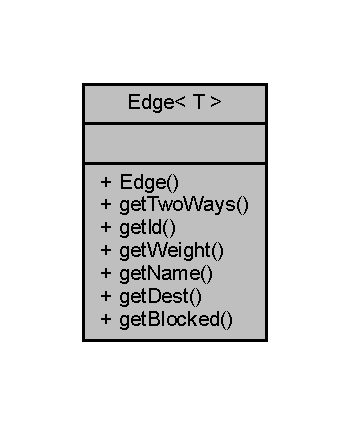
\includegraphics[width=168pt]{class_edge__coll__graph}
\end{center}
\end{figure}
\subsection*{Membros públicos}
\begin{DoxyCompactItemize}
\item 
\hyperlink{class_edge_aa83400a85aa2e50327bdc8ba854ad375}{Edge} (\hyperlink{class_vertex}{Vertex}$<$ T $>$ $\ast$d, double w, bool tw, bool block, T id, string name)
\item 
bool \hyperlink{class_edge_a330979d3f8be8f4f26889e046adf5eb2}{get\+Two\+Ways} () const 
\item 
T \hyperlink{class_edge_a655569c8bc3e9154d82a49ffebf0a8e6}{get\+Id} () const 
\item 
int \hyperlink{class_edge_a9c0f42ab235c2c427d2239bf5419b854}{get\+Weight} () const 
\item 
string \hyperlink{class_edge_a29153ede6a73b12918e3c05a9532cf4e}{get\+Name} () const 
\item 
\hyperlink{class_vertex}{Vertex}$<$ T $>$ $\ast$ \hyperlink{class_edge_a3805fa2e04f1e7f0495fbba6524ea823}{get\+Dest} () const 
\item 
bool \hyperlink{class_edge_a6b46f098c5d22a74ee404f34dd89c0eb}{get\+Blocked} () const 
\end{DoxyCompactItemize}
\subsection*{Amigos}
\begin{DoxyCompactItemize}
\item 
class \hyperlink{class_edge_aefa9b76cd57411c5354e5620dc2d84dd}{Graph$<$ T $>$}
\item 
class \hyperlink{class_edge_a2e120a12dec663fa334633b4f26cbed8}{Vertex$<$ T $>$}
\end{DoxyCompactItemize}


\subsection{Documentação dos Construtores \& Destrutor}
\hypertarget{class_edge_aa83400a85aa2e50327bdc8ba854ad375}{}\index{Edge@{Edge}!Edge@{Edge}}
\index{Edge@{Edge}!Edge@{Edge}}
\subsubsection[{Edge(\+Vertex$<$ T $>$ $\ast$d, double w, bool tw, bool block, T id, string name)}]{\setlength{\rightskip}{0pt plus 5cm}template$<$class T $>$ {\bf Edge}$<$ T $>$\+::{\bf Edge} (
\begin{DoxyParamCaption}
\item[{{\bf Vertex}$<$ T $>$ $\ast$}]{d, }
\item[{double}]{w, }
\item[{bool}]{tw, }
\item[{bool}]{block, }
\item[{T}]{id, }
\item[{string}]{name}
\end{DoxyParamCaption}
)}\label{class_edge_aa83400a85aa2e50327bdc8ba854ad375}


\subsection{Documentação dos métodos}
\hypertarget{class_edge_a6b46f098c5d22a74ee404f34dd89c0eb}{}\index{Edge@{Edge}!get\+Blocked@{get\+Blocked}}
\index{get\+Blocked@{get\+Blocked}!Edge@{Edge}}
\subsubsection[{get\+Blocked() const }]{\setlength{\rightskip}{0pt plus 5cm}template$<$class T $>$ bool {\bf Edge}$<$ T $>$\+::get\+Blocked (
\begin{DoxyParamCaption}
{}
\end{DoxyParamCaption}
) const}\label{class_edge_a6b46f098c5d22a74ee404f34dd89c0eb}
\hypertarget{class_edge_a3805fa2e04f1e7f0495fbba6524ea823}{}\index{Edge@{Edge}!get\+Dest@{get\+Dest}}
\index{get\+Dest@{get\+Dest}!Edge@{Edge}}
\subsubsection[{get\+Dest() const }]{\setlength{\rightskip}{0pt plus 5cm}template$<$class T $>$ {\bf Vertex}$<$ T $>$ $\ast$ {\bf Edge}$<$ T $>$\+::get\+Dest (
\begin{DoxyParamCaption}
{}
\end{DoxyParamCaption}
) const}\label{class_edge_a3805fa2e04f1e7f0495fbba6524ea823}
\hypertarget{class_edge_a655569c8bc3e9154d82a49ffebf0a8e6}{}\index{Edge@{Edge}!get\+Id@{get\+Id}}
\index{get\+Id@{get\+Id}!Edge@{Edge}}
\subsubsection[{get\+Id() const }]{\setlength{\rightskip}{0pt plus 5cm}template$<$class T $>$ T {\bf Edge}$<$ T $>$\+::get\+Id (
\begin{DoxyParamCaption}
{}
\end{DoxyParamCaption}
) const}\label{class_edge_a655569c8bc3e9154d82a49ffebf0a8e6}
\hypertarget{class_edge_a29153ede6a73b12918e3c05a9532cf4e}{}\index{Edge@{Edge}!get\+Name@{get\+Name}}
\index{get\+Name@{get\+Name}!Edge@{Edge}}
\subsubsection[{get\+Name() const }]{\setlength{\rightskip}{0pt plus 5cm}template$<$class T $>$ string {\bf Edge}$<$ T $>$\+::get\+Name (
\begin{DoxyParamCaption}
{}
\end{DoxyParamCaption}
) const}\label{class_edge_a29153ede6a73b12918e3c05a9532cf4e}
\hypertarget{class_edge_a330979d3f8be8f4f26889e046adf5eb2}{}\index{Edge@{Edge}!get\+Two\+Ways@{get\+Two\+Ways}}
\index{get\+Two\+Ways@{get\+Two\+Ways}!Edge@{Edge}}
\subsubsection[{get\+Two\+Ways() const }]{\setlength{\rightskip}{0pt plus 5cm}template$<$class T $>$ bool {\bf Edge}$<$ T $>$\+::get\+Two\+Ways (
\begin{DoxyParamCaption}
{}
\end{DoxyParamCaption}
) const}\label{class_edge_a330979d3f8be8f4f26889e046adf5eb2}
\hypertarget{class_edge_a9c0f42ab235c2c427d2239bf5419b854}{}\index{Edge@{Edge}!get\+Weight@{get\+Weight}}
\index{get\+Weight@{get\+Weight}!Edge@{Edge}}
\subsubsection[{get\+Weight() const }]{\setlength{\rightskip}{0pt plus 5cm}template$<$class T $>$ int {\bf Edge}$<$ T $>$\+::get\+Weight (
\begin{DoxyParamCaption}
{}
\end{DoxyParamCaption}
) const}\label{class_edge_a9c0f42ab235c2c427d2239bf5419b854}


\subsection{Documentação das classes amigas e funções relacionadas}
\hypertarget{class_edge_aefa9b76cd57411c5354e5620dc2d84dd}{}\index{Edge@{Edge}!Graph$<$ T $>$@{Graph$<$ T $>$}}
\index{Graph$<$ T $>$@{Graph$<$ T $>$}!Edge@{Edge}}
\subsubsection[{Graph$<$ T $>$}]{\setlength{\rightskip}{0pt plus 5cm}template$<$class T$>$ friend class {\bf Graph}$<$ T $>$\hspace{0.3cm}{\ttfamily [friend]}}\label{class_edge_aefa9b76cd57411c5354e5620dc2d84dd}
\hypertarget{class_edge_a2e120a12dec663fa334633b4f26cbed8}{}\index{Edge@{Edge}!Vertex$<$ T $>$@{Vertex$<$ T $>$}}
\index{Vertex$<$ T $>$@{Vertex$<$ T $>$}!Edge@{Edge}}
\subsubsection[{Vertex$<$ T $>$}]{\setlength{\rightskip}{0pt plus 5cm}template$<$class T$>$ friend class {\bf Vertex}$<$ T $>$\hspace{0.3cm}{\ttfamily [friend]}}\label{class_edge_a2e120a12dec663fa334633b4f26cbed8}


A documentação para esta classe foi gerada a partir do seguinte ficheiro\+:\begin{DoxyCompactItemize}
\item 
C\+:/\+Users/josea/\+Documents/\+Git\+Hub/\+C\+A\+L-\/\+Easy\+Pilot/\+Easy\+Pilot/src/\hyperlink{_graph_8h}{Graph.\+h}\end{DoxyCompactItemize}

\hypertarget{class_edge_type}{}\section{Referência à classe Edge\+Type}
\label{class_edge_type}\index{Edge\+Type@{Edge\+Type}}


{\ttfamily \#include $<$edgetype.\+h$>$}



Diagrama de colaboração para Edge\+Type\+:
\nopagebreak
\begin{figure}[H]
\begin{center}
\leavevmode
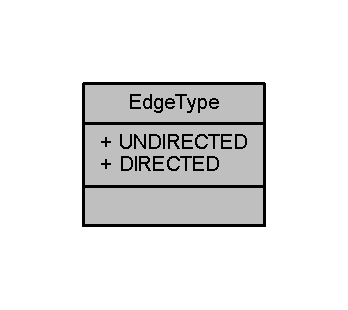
\includegraphics[width=167pt]{class_edge_type__coll__graph}
\end{center}
\end{figure}
\subsection*{Atributos Públicos Estáticos}
\begin{DoxyCompactItemize}
\item 
\hypertarget{class_edge_type_a6533cc56d05c288a550b9980b66c9317}{}static const int {\bfseries U\+N\+D\+I\+R\+E\+C\+T\+E\+D} = 0\label{class_edge_type_a6533cc56d05c288a550b9980b66c9317}

\item 
\hypertarget{class_edge_type_a903017a534f2818c2d17145e4ae0321c}{}static const int {\bfseries D\+I\+R\+E\+C\+T\+E\+D} = 1\label{class_edge_type_a903017a534f2818c2d17145e4ae0321c}

\end{DoxyCompactItemize}


\subsection{Descrição detalhada}
Classe que enumera os tipos de arestas. Usar Edge\+Type.\+U\+N\+D\+I\+R\+E\+C\+T\+E\+D para uma aresta sem direcção, ou Edge\+Type.\+D\+I\+R\+E\+C\+T\+E\+D para uma aresta dirigida. 

A documentação para esta classe foi gerada a partir do seguinte ficheiro\+:\begin{DoxyCompactItemize}
\item 
C\+:/\+Users/josea/\+Documents/\+Git\+Hub/\+C\+A\+L-\/\+Proj/\+Easy\+Pilot/src/edgetype.\+h\end{DoxyCompactItemize}

\hypertarget{class_graph}{}\section{Referência à classe Template Graph$<$ T $>$}
\label{class_graph}\index{Graph$<$ T $>$@{Graph$<$ T $>$}}


Diagrama de colaboração para Graph$<$ T $>$\+:
\nopagebreak
\begin{figure}[H]
\begin{center}
\leavevmode
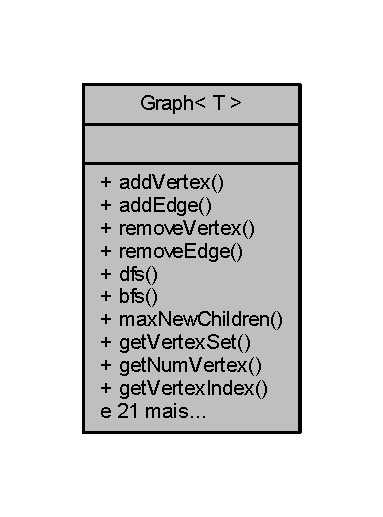
\includegraphics[width=184pt]{class_graph__coll__graph}
\end{center}
\end{figure}
\subsection*{Membros públicos}
\begin{DoxyCompactItemize}
\item 
\hypertarget{class_graph_a6283650774199e3dc971f226eb35cf50}{}bool {\bfseries add\+Vertex} (const T \&in, double longitude, double latitude)\label{class_graph_a6283650774199e3dc971f226eb35cf50}

\item 
\hypertarget{class_graph_add7835e0874b6bb515980db864e39a86}{}bool {\bfseries add\+Edge} (const T \&sourc, const T \&dest, double w, bool tw, bool blocked, T id, string name)\label{class_graph_add7835e0874b6bb515980db864e39a86}

\item 
\hypertarget{class_graph_af9c903104ad69a7782979fa9caedf163}{}bool {\bfseries remove\+Vertex} (const T \&in)\label{class_graph_af9c903104ad69a7782979fa9caedf163}

\item 
\hypertarget{class_graph_a1106092a37366486cf55576f9ec01692}{}bool {\bfseries remove\+Edge} (const T \&sourc, const T \&dest)\label{class_graph_a1106092a37366486cf55576f9ec01692}

\item 
\hypertarget{class_graph_a3f62ba0e37c5c011299c93d60e3a8be3}{}vector$<$ T $>$ {\bfseries dfs} () const \label{class_graph_a3f62ba0e37c5c011299c93d60e3a8be3}

\item 
\hypertarget{class_graph_a0e9598b98be2570eb432690411a577e8}{}vector$<$ T $>$ {\bfseries bfs} (\hyperlink{class_vertex}{Vertex}$<$ T $>$ $\ast$v) const \label{class_graph_a0e9598b98be2570eb432690411a577e8}

\item 
\hypertarget{class_graph_ab8fd74c3cf8dca6eaa82d39fd1216f52}{}int {\bfseries max\+New\+Children} (\hyperlink{class_vertex}{Vertex}$<$ T $>$ $\ast$v, T \&inf) const \label{class_graph_ab8fd74c3cf8dca6eaa82d39fd1216f52}

\item 
\hypertarget{class_graph_ab7dc5ec1c34df811d560021b726e95ec}{}vector$<$ \hyperlink{class_vertex}{Vertex}$<$ T $>$ $\ast$ $>$ {\bfseries get\+Vertex\+Set} () const \label{class_graph_ab7dc5ec1c34df811d560021b726e95ec}

\item 
\hypertarget{class_graph_a295932f117d92c825a97ec458e0fb332}{}int {\bfseries get\+Num\+Vertex} () const \label{class_graph_a295932f117d92c825a97ec458e0fb332}

\item 
\hypertarget{class_graph_a98ad6f08d48ceb7527cb37433c0efc56}{}int {\bfseries get\+Vertex\+Index} (const T \&v) const \label{class_graph_a98ad6f08d48ceb7527cb37433c0efc56}

\item 
int \hyperlink{class_graph_a41708134b9e518beea032e6e62d84bef}{calculate\+Edge\+Weight} (T id1, T id2) const 
\item 
void \hyperlink{class_graph_a7b9a7f15067572593b8be54c59ac1b32}{apply\+Toll\+Weight} (\hyperlink{class_toll}{Toll} \&t, \hyperlink{class_graph_viewer}{Graph\+Viewer} $\ast$gv)
\begin{DoxyCompactList}\small\item\em Takes a toll and applies a change of weight to all its adjacent edges, according to its cost. It adds 100$\ast$cost to the weight of the edge. \end{DoxyCompactList}\item 
\hypertarget{class_graph_adbb6e61a997bdd22911d5f38361d38bd}{}void {\bfseries remove\+Toll\+Weight} (\hyperlink{class_toll}{Toll} \&t, \hyperlink{class_graph_viewer}{Graph\+Viewer} $\ast$gv)\label{class_graph_adbb6e61a997bdd22911d5f38361d38bd}

\item 
\hypertarget{class_graph_a08a95472b0d9bd7321660940807af060}{}\hyperlink{class_vertex}{Vertex}$<$ T $>$ $\ast$ {\bfseries get\+Vertex} (const T \&v) const \label{class_graph_a08a95472b0d9bd7321660940807af060}

\item 
\hypertarget{class_graph_a45b90c42b1fd441a721cb3af43d07f07}{}\hyperlink{class_edge}{Edge}$<$ T $>$ $\ast$ {\bfseries get\+Edge} (const T \&v) const \label{class_graph_a45b90c42b1fd441a721cb3af43d07f07}

\item 
\hypertarget{class_graph_af34eb86d804272e6e3e221a9ed688c53}{}void {\bfseries reset\+Indegrees} ()\label{class_graph_af34eb86d804272e6e3e221a9ed688c53}

\item 
\hypertarget{class_graph_aa1a3c754f51a888e25dff2b26dfb85fc}{}vector$<$ \hyperlink{class_vertex}{Vertex}$<$ T $>$ $\ast$ $>$ {\bfseries get\+Sources} () const \label{class_graph_aa1a3c754f51a888e25dff2b26dfb85fc}

\item 
\hypertarget{class_graph_a694dff81073c38b669057f0c6bd4cbb1}{}int {\bfseries get\+Num\+Cycles} ()\label{class_graph_a694dff81073c38b669057f0c6bd4cbb1}

\item 
\hypertarget{class_graph_a2e75512c089c3916dda9cf61e1185d9d}{}vector$<$ T $>$ {\bfseries topological\+Order} ()\label{class_graph_a2e75512c089c3916dda9cf61e1185d9d}

\item 
\hypertarget{class_graph_ab4054ca572c10669dd3e05d6d41c116c}{}vector$<$ T $>$ {\bfseries get\+Path} (const T \&origin, const T \&dest)\label{class_graph_ab4054ca572c10669dd3e05d6d41c116c}

\item 
\hypertarget{class_graph_ae5264597aacaf4f45819e96a6d6c89aa}{}void {\bfseries unweighted\+Shortest\+Path} (const T \&v)\label{class_graph_ae5264597aacaf4f45819e96a6d6c89aa}

\item 
\hypertarget{class_graph_ab49d07c2bd6b8b30d5ae82bc558b821a}{}bool {\bfseries is\+D\+A\+G} ()\label{class_graph_ab49d07c2bd6b8b30d5ae82bc558b821a}

\item 
\hypertarget{class_graph_a1d6769b79beaa76f78fd9c9209833bef}{}void {\bfseries bellman\+Ford\+Shortest\+Path} (const T \&s)\label{class_graph_a1d6769b79beaa76f78fd9c9209833bef}

\item 
\hypertarget{class_graph_a445a38cf4045797198eae2b818b602de}{}void {\bfseries dijkstra\+Shortest\+Path} (const T \&s)\label{class_graph_a445a38cf4045797198eae2b818b602de}

\item 
\hypertarget{class_graph_ae5161f4408bf1ead2b29d19d67fb04ee}{}void {\bfseries floyd\+Warshall\+Shortest\+Path} ()\label{class_graph_ae5161f4408bf1ead2b29d19d67fb04ee}

\item 
\hypertarget{class_graph_a7e137f1ef838395ac1044a944fa54448}{}int {\bfseries edge\+Cost} (int v\+Orig\+Index, int v\+Dest\+Index)\label{class_graph_a7e137f1ef838395ac1044a944fa54448}

\item 
\hypertarget{class_graph_ab23d1dae92a7f2b29dcb91a94336674c}{}vector$<$ T $>$ {\bfseries getfloyd\+Warshall\+Path} (const T \&origin, const T \&dest)\label{class_graph_ab23d1dae92a7f2b29dcb91a94336674c}

\item 
\hypertarget{class_graph_aad1eda4beb8425d03ed1f3b8af397563}{}void {\bfseries getfloyd\+Warshall\+Path\+Aux} (int index1, int index2, vector$<$ T $>$ \&res)\label{class_graph_aad1eda4beb8425d03ed1f3b8af397563}

\item 
\hypertarget{class_graph_ad10eead5afadfb05a78fd8dd606238f8}{}int {\bfseries get\+Num\+Edge} () const \label{class_graph_ad10eead5afadfb05a78fd8dd606238f8}

\item 
\hypertarget{class_graph_a18b0ca37a9f279089a71aa5c3ba16e1e}{}void {\bfseries clear\+Graph} ()\label{class_graph_a18b0ca37a9f279089a71aa5c3ba16e1e}

\item 
\hypertarget{class_graph_a338f11555225fc082d5f5777cfd2e01d}{}void {\bfseries set\+Edge\+Blocked} (const T \&v, bool b)\label{class_graph_a338f11555225fc082d5f5777cfd2e01d}

\end{DoxyCompactItemize}


\subsection{Documentação dos métodos}
\hypertarget{class_graph_a7b9a7f15067572593b8be54c59ac1b32}{}\index{Graph@{Graph}!apply\+Toll\+Weight@{apply\+Toll\+Weight}}
\index{apply\+Toll\+Weight@{apply\+Toll\+Weight}!Graph@{Graph}}
\subsubsection[{apply\+Toll\+Weight(\+Toll \&t, Graph\+Viewer $\ast$gv)}]{\setlength{\rightskip}{0pt plus 5cm}template$<$class T $>$ void {\bf Graph}$<$ T $>$\+::apply\+Toll\+Weight (
\begin{DoxyParamCaption}
\item[{{\bf Toll} \&}]{t, }
\item[{{\bf Graph\+Viewer} $\ast$}]{gv}
\end{DoxyParamCaption}
)}\label{class_graph_a7b9a7f15067572593b8be54c59ac1b32}


Takes a toll and applies a change of weight to all its adjacent edges, according to its cost. It adds 100$\ast$cost to the weight of the edge. 


\begin{DoxyParams}{Parâmetros}
{\em \hyperlink{class_toll}{Toll}} & t \hyperlink{class_toll}{Toll} to be applied. \\
\hline
\end{DoxyParams}
\hypertarget{class_graph_a41708134b9e518beea032e6e62d84bef}{}\index{Graph@{Graph}!calculate\+Edge\+Weight@{calculate\+Edge\+Weight}}
\index{calculate\+Edge\+Weight@{calculate\+Edge\+Weight}!Graph@{Graph}}
\subsubsection[{calculate\+Edge\+Weight(\+T id1, T id2) const }]{\setlength{\rightskip}{0pt plus 5cm}template$<$class T$>$ int {\bf Graph}$<$ T $>$\+::calculate\+Edge\+Weight (
\begin{DoxyParamCaption}
\item[{T}]{id1, }
\item[{T}]{id2}
\end{DoxyParamCaption}
) const}\label{class_graph_a41708134b9e518beea032e6e62d84bef}
Calculates an edge weight according to the distance that separates its nodes. The applied formula is the distance between the two points times 1000, so it has a significant amount of weight.


\begin{DoxyParams}{Parâmetros}
{\em T} & id1 Content of node 1. \\
\hline
{\em T} & id2 Content of node 2. \\
\hline
\end{DoxyParams}


A documentação para esta classe foi gerada a partir do seguinte ficheiro\+:\begin{DoxyCompactItemize}
\item 
C\+:/\+Users/josea/\+Documents/\+Git\+Hub/\+C\+A\+L-\/\+Proj/\+Easy\+Pilot/src/Graph.\+h\end{DoxyCompactItemize}

\hypertarget{class_graph_viewer}{}\section{Referência à classe Graph\+Viewer}
\label{class_graph_viewer}\index{Graph\+Viewer@{Graph\+Viewer}}


{\ttfamily \#include $<$graphviewer.\+h$>$}



Diagrama de colaboração para Graph\+Viewer\+:
\nopagebreak
\begin{figure}[H]
\begin{center}
\leavevmode
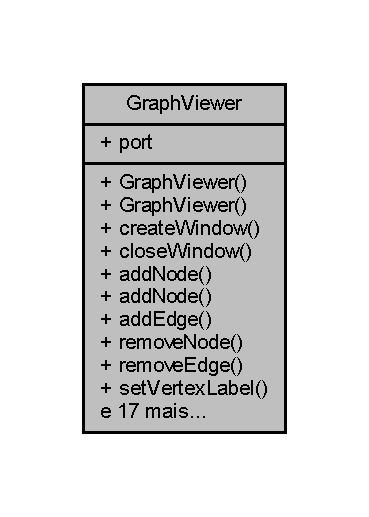
\includegraphics[width=177pt]{class_graph_viewer__coll__graph}
\end{center}
\end{figure}
\subsection*{Membros públicos}
\begin{DoxyCompactItemize}
\item 
\hyperlink{class_graph_viewer_a8adc614f4fc290a3efcec7d7ceb1c58a}{Graph\+Viewer} (int width, int height, bool dynamic)
\item 
\hyperlink{class_graph_viewer_ad9d7b1d8b4ba8ef18517eae0e68568a2}{Graph\+Viewer} (int width, int height, bool dynamic, int port\+\_\+n)
\item 
bool \hyperlink{class_graph_viewer_ae5247dc66449dcd21fc5d531bbbaddfa}{create\+Window} (int width, int height)
\item 
bool \hyperlink{class_graph_viewer_a85990c1eaac7feed3950960d4bd2fd4c}{close\+Window} ()
\item 
bool \hyperlink{class_graph_viewer_a5421e86ac76433876309236ba96e70a2}{add\+Node} (int id, int x, int y)
\item 
bool \hyperlink{class_graph_viewer_ab9be856eb5f45284719a3bb119ec01ea}{add\+Node} (int id)
\item 
bool \hyperlink{class_graph_viewer_aad0c1448c37f744209ffb671f1bd0015}{add\+Edge} (int id, int v1, int v2, int edge\+Type)
\item 
bool \hyperlink{class_graph_viewer_a0c418639bb911eb827cabf895915f775}{remove\+Node} (int id)
\item 
bool \hyperlink{class_graph_viewer_a9a8ee68c7c12b373affbe4069dd95d72}{remove\+Edge} (int id)
\item 
bool \hyperlink{class_graph_viewer_ac25d7d007022fda16799808ba136e909}{set\+Vertex\+Label} (int id, string label)
\item 
bool \hyperlink{class_graph_viewer_a447cca0064e785654c2105602c2961ca}{set\+Edge\+Label} (int id, string label)
\item 
bool \hyperlink{class_graph_viewer_a07ccc96707efae4aa5f3ced3dca015af}{set\+Edge\+Color} (int id, string color)
\item 
bool \hyperlink{class_graph_viewer_a1698f1c6b3a8e7cabc7b7d7cf42fc7f0}{set\+Edge\+Dashed} (int id, bool dashed)
\item 
bool \hyperlink{class_graph_viewer_a8b542d7e09e81a45a74760c19233beb0}{set\+Vertex\+Color} (int id, string color)
\item 
bool \hyperlink{class_graph_viewer_ae930dfdfcdeb7a871eefb6028d74b9f9}{set\+Vertex\+Size} (int id, int size)
\item 
bool \hyperlink{class_graph_viewer_a02d5f7393eab9a2d1b66719039597a64}{set\+Vertex\+Icon} (int id, string filepath)
\item 
bool \hyperlink{class_graph_viewer_a07f598272fe3515455eab13be749604a}{set\+Edge\+Thickness} (int id, int thickness)
\item 
bool \hyperlink{class_graph_viewer_ac211de009a0afe2e6d44f4f8d030a2cc}{set\+Edge\+Weight} (int id, int weight)
\item 
bool \hyperlink{class_graph_viewer_a69eb065145063e4dea41961e92e35c8e}{set\+Edge\+Flow} (int id, int flow)
\item 
bool \hyperlink{class_graph_viewer_a08f362be0e682d91e7506dca8caae1b8}{define\+Edge\+Curved} (bool curved)
\item 
bool \hyperlink{class_graph_viewer_a4102580b69826ba83251ef7bb262f8be}{define\+Edge\+Color} (string color)
\item 
bool \hyperlink{class_graph_viewer_af785279b5c204df0e274b20c36276fc3}{define\+Edge\+Dashed} (bool dashed)
\item 
bool \hyperlink{class_graph_viewer_a76de8676b7a93d72af514b84cdaa4d21}{define\+Vertex\+Color} (string color)
\item 
bool \hyperlink{class_graph_viewer_ac4b2a9fec74d38e64088aa79ca4b7d9b}{define\+Vertex\+Size} (int size)
\item 
bool \hyperlink{class_graph_viewer_af1adb6a361457187a820e01dcf0a34b7}{define\+Vertex\+Icon} (string filepath)
\item 
bool \hyperlink{class_graph_viewer_a02437b5fecd8b90de24436068312d593}{set\+Background} (string path)
\item 
bool \hyperlink{class_graph_viewer_a3009a66958686ccb7e78b68e37c3c423}{rearrange} ()
\end{DoxyCompactItemize}
\subsection*{Atributos Públicos Estáticos}
\begin{DoxyCompactItemize}
\item 
static short \hyperlink{class_graph_viewer_a89d0abe75f41feededc49497cc514342}{port} = 7772
\end{DoxyCompactItemize}


\subsection{Descrição detalhada}
Classe que guarda o grafo e o representa. Todas as suas funções retornam um booleano a indicar se a sua execução decorreu ou não com sucesso. 

\subsection{Documentação dos Construtores \& Destrutor}
\hypertarget{class_graph_viewer_a8adc614f4fc290a3efcec7d7ceb1c58a}{}\index{Graph\+Viewer@{Graph\+Viewer}!Graph\+Viewer@{Graph\+Viewer}}
\index{Graph\+Viewer@{Graph\+Viewer}!Graph\+Viewer@{Graph\+Viewer}}
\subsubsection[{Graph\+Viewer(int width, int height, bool dynamic)}]{\setlength{\rightskip}{0pt plus 5cm}Graph\+Viewer\+::\+Graph\+Viewer (
\begin{DoxyParamCaption}
\item[{int}]{width, }
\item[{int}]{height, }
\item[{bool}]{dynamic}
\end{DoxyParamCaption}
)}\label{class_graph_viewer_a8adc614f4fc290a3efcec7d7ceb1c58a}
Construtor que cria um novo grafo e atribui automaticamente a porta. Exemplo\+: \hyperlink{class_graph_viewer}{Graph\+Viewer} $\ast$gv = new \hyperlink{class_graph_viewer}{Graph\+Viewer(600, 600, true)}; instancia um grafo 600x600, onde a posição dos nós é determinada automaticamente.


\begin{DoxyParams}{Parâmetros}
{\em width} & Inteiro que representa a lagura da área do grafo. \\
\hline
{\em height} & Inteiro que representa a altura da área do grafo. \\
\hline
{\em dynamic} & Booleano que determina se a localização dos nós é automaticamente. determinado pelo programa (true) ou se deve ser determinado pelo utilizador (false). \\
\hline
\end{DoxyParams}
\hypertarget{class_graph_viewer_ad9d7b1d8b4ba8ef18517eae0e68568a2}{}\index{Graph\+Viewer@{Graph\+Viewer}!Graph\+Viewer@{Graph\+Viewer}}
\index{Graph\+Viewer@{Graph\+Viewer}!Graph\+Viewer@{Graph\+Viewer}}
\subsubsection[{Graph\+Viewer(int width, int height, bool dynamic, int port\+\_\+n)}]{\setlength{\rightskip}{0pt plus 5cm}Graph\+Viewer\+::\+Graph\+Viewer (
\begin{DoxyParamCaption}
\item[{int}]{width, }
\item[{int}]{height, }
\item[{bool}]{dynamic, }
\item[{int}]{port\+\_\+n}
\end{DoxyParamCaption}
)}\label{class_graph_viewer_ad9d7b1d8b4ba8ef18517eae0e68568a2}
Construtor que cria um novo grafo, utilizando uma porta especificada pelo utilizador para a ligação.

Exemplo\+: \hyperlink{class_graph_viewer}{Graph\+Viewer} $\ast$gv = new \hyperlink{class_graph_viewer}{Graph\+Viewer(600, 600, false, 3000)}; instancia um grafo 600x600, onde a posição dos nós é determinada pelo utilizador (usando a versão de add\+Node onde se pode especificar as coordenadas), sendo que a porta a usar para a comunicação é a 3000.


\begin{DoxyParams}{Parâmetros}
{\em width} & Inteiro que representa a lagura da área do grafo. \\
\hline
{\em height} & Inteiro que representa a altura da área do grafo. \\
\hline
{\em dynamic} & Booleano que determina se a localização dos nós é automaticamente. determinado pelo programa (true) ou se deve ser determinado pelo utilizador (false). \\
\hline
{\em port\+\_\+n} & Inteiro que determina a porta a utilizar. Deve-\/se ter cuidado para não utilizar uma porta já usada por outro programa ou pelo sistema. \\
\hline
\end{DoxyParams}


\subsection{Documentação dos métodos}
\hypertarget{class_graph_viewer_aad0c1448c37f744209ffb671f1bd0015}{}\index{Graph\+Viewer@{Graph\+Viewer}!add\+Edge@{add\+Edge}}
\index{add\+Edge@{add\+Edge}!Graph\+Viewer@{Graph\+Viewer}}
\subsubsection[{add\+Edge(int id, int v1, int v2, int edge\+Type)}]{\setlength{\rightskip}{0pt plus 5cm}bool Graph\+Viewer\+::add\+Edge (
\begin{DoxyParamCaption}
\item[{int}]{id, }
\item[{int}]{v1, }
\item[{int}]{v2, }
\item[{int}]{edge\+Type}
\end{DoxyParamCaption}
)}\label{class_graph_viewer_aad0c1448c37f744209ffb671f1bd0015}
Acrescenta uma aresta à representação do grafo. Exemplo, para um apontador gv onde foi instanciada a classe \hyperlink{class_graph_viewer}{Graph\+Viewer}\+: gv-\/$>$add\+Edge(0, 1, 2, Edge\+Type\+::\+U\+N\+D\+I\+R\+E\+C\+T\+E\+D); adiciona uma aresta não-\/dirigida com I\+D 0 que liga os nós com os I\+Ds 1 e 2


\begin{DoxyParams}{Parâmetros}
{\em id} & Identificador único da aresta. \\
\hline
{\em v1} & Identificador único do nó de origem da aresta. \\
\hline
{\em v2} & Identificador único do nó de destino da aresta. \\
\hline
{\em edge\+Type} & Edge\+Type.\+D\+I\+R\+E\+C\+T\+E\+D caso a aresta seja unidirecional ou Edge\+Type.\+U\+N\+D\+I\+R\+E\+C\+T\+E\+D caso a aresta seja bidirecional. \\
\hline
\end{DoxyParams}
\hypertarget{class_graph_viewer_a5421e86ac76433876309236ba96e70a2}{}\index{Graph\+Viewer@{Graph\+Viewer}!add\+Node@{add\+Node}}
\index{add\+Node@{add\+Node}!Graph\+Viewer@{Graph\+Viewer}}
\subsubsection[{add\+Node(int id, int x, int y)}]{\setlength{\rightskip}{0pt plus 5cm}bool Graph\+Viewer\+::add\+Node (
\begin{DoxyParamCaption}
\item[{int}]{id, }
\item[{int}]{x, }
\item[{int}]{y}
\end{DoxyParamCaption}
)}\label{class_graph_viewer_a5421e86ac76433876309236ba96e70a2}
Acrescenta um nó à representação do grafo, numa posição específica, irrelevante se o grafo for dinâmico. Exemplo, para um apontador gv onde foi instanciada a classe \hyperlink{class_graph_viewer}{Graph\+Viewer} com is\+Dynamic = false\+: gv-\/$>$add\+Node(0, 1, 2); adiciona um nó com I\+D 0 na posição (x, y) = (1, 2)


\begin{DoxyParams}{Parâmetros}
{\em id} & Identificador único do nó. \\
\hline
{\em x} & Posição horizontal do nó. \\
\hline
{\em y} & Posição vertical do nó. \\
\hline
\end{DoxyParams}
\hypertarget{class_graph_viewer_ab9be856eb5f45284719a3bb119ec01ea}{}\index{Graph\+Viewer@{Graph\+Viewer}!add\+Node@{add\+Node}}
\index{add\+Node@{add\+Node}!Graph\+Viewer@{Graph\+Viewer}}
\subsubsection[{add\+Node(int id)}]{\setlength{\rightskip}{0pt plus 5cm}bool Graph\+Viewer\+::add\+Node (
\begin{DoxyParamCaption}
\item[{int}]{id}
\end{DoxyParamCaption}
)}\label{class_graph_viewer_ab9be856eb5f45284719a3bb119ec01ea}
Acrescenta um nó à representação do grafo, numa posição ao critério do programa. Só pode ser usado se o grafo for dinâmico, ou seja, se as posições de todos os nós forem atribuídas automaticamente. Caso contrário, não adiciona o nó. Exemplo, para um apontador gv onde foi instanciada a classe \hyperlink{class_graph_viewer}{Graph\+Viewer} com is\+Dynamic = true\+: gv-\/$>$add\+Node(0); adiciona um nó com I\+D 0


\begin{DoxyParams}{Parâmetros}
{\em id} & Identificador único do nó. \\
\hline
\end{DoxyParams}
\hypertarget{class_graph_viewer_a85990c1eaac7feed3950960d4bd2fd4c}{}\index{Graph\+Viewer@{Graph\+Viewer}!close\+Window@{close\+Window}}
\index{close\+Window@{close\+Window}!Graph\+Viewer@{Graph\+Viewer}}
\subsubsection[{close\+Window()}]{\setlength{\rightskip}{0pt plus 5cm}bool Graph\+Viewer\+::close\+Window (
\begin{DoxyParamCaption}
{}
\end{DoxyParamCaption}
)}\label{class_graph_viewer_a85990c1eaac7feed3950960d4bd2fd4c}
Fecha a janela a ser utilizada para visualização. \hypertarget{class_graph_viewer_ae5247dc66449dcd21fc5d531bbbaddfa}{}\index{Graph\+Viewer@{Graph\+Viewer}!create\+Window@{create\+Window}}
\index{create\+Window@{create\+Window}!Graph\+Viewer@{Graph\+Viewer}}
\subsubsection[{create\+Window(int width, int height)}]{\setlength{\rightskip}{0pt plus 5cm}bool Graph\+Viewer\+::create\+Window (
\begin{DoxyParamCaption}
\item[{int}]{width, }
\item[{int}]{height}
\end{DoxyParamCaption}
)}\label{class_graph_viewer_ae5247dc66449dcd21fc5d531bbbaddfa}
Função que cria a janela para visualização. Exemplo, para um apontador gv onde foi instanciada a classe \hyperlink{class_graph_viewer}{Graph\+Viewer}\+: gv-\/$>$create\+Window(600, 600); abre uma janela 600x600 onde mostra o grafo.


\begin{DoxyParams}{Parâmetros}
{\em width} & Largura da janela a criar. \\
\hline
{\em height} & Altura da janela a criar. \\
\hline
\end{DoxyParams}
\hypertarget{class_graph_viewer_a4102580b69826ba83251ef7bb262f8be}{}\index{Graph\+Viewer@{Graph\+Viewer}!define\+Edge\+Color@{define\+Edge\+Color}}
\index{define\+Edge\+Color@{define\+Edge\+Color}!Graph\+Viewer@{Graph\+Viewer}}
\subsubsection[{define\+Edge\+Color(string color)}]{\setlength{\rightskip}{0pt plus 5cm}bool Graph\+Viewer\+::define\+Edge\+Color (
\begin{DoxyParamCaption}
\item[{string}]{color}
\end{DoxyParamCaption}
)}\label{class_graph_viewer_a4102580b69826ba83251ef7bb262f8be}
Função que define a cor global das arestas. Exemplo, para um apontador gv onde foi instanciada a classe \hyperlink{class_graph_viewer}{Graph\+Viewer}\+: gv-\/$>$define\+Edge\+Color(\+G\+R\+A\+Y); modifica a cor por defeito das arestas para cinzento


\begin{DoxyParams}{Parâmetros}
{\em color} & Nova cor das arestas, utilizar as constantes definidas no \hyperlink{graphviewer_8h_source}{graphviewer.\+h} para conveniência. \\
\hline
\end{DoxyParams}
\hypertarget{class_graph_viewer_a08f362be0e682d91e7506dca8caae1b8}{}\index{Graph\+Viewer@{Graph\+Viewer}!define\+Edge\+Curved@{define\+Edge\+Curved}}
\index{define\+Edge\+Curved@{define\+Edge\+Curved}!Graph\+Viewer@{Graph\+Viewer}}
\subsubsection[{define\+Edge\+Curved(bool curved)}]{\setlength{\rightskip}{0pt plus 5cm}bool Graph\+Viewer\+::define\+Edge\+Curved (
\begin{DoxyParamCaption}
\item[{bool}]{curved}
\end{DoxyParamCaption}
)}\label{class_graph_viewer_a08f362be0e682d91e7506dca8caae1b8}
Função que define se as arestas do grafo serão desenhadas como curvas ou retas. Exemplo, para um apontador gv onde foi instanciada a classe \hyperlink{class_graph_viewer}{Graph\+Viewer}\+: gv-\/$>$define\+Edge\+Curved(false); faz com que as arestas sejam desenhadas como retas


\begin{DoxyParams}{Parâmetros}
{\em curved} & Booleano que representa se as arestas serão curvas (true) ou retas (false), sendo o valor por defeito é true. \\
\hline
\end{DoxyParams}
\hypertarget{class_graph_viewer_af785279b5c204df0e274b20c36276fc3}{}\index{Graph\+Viewer@{Graph\+Viewer}!define\+Edge\+Dashed@{define\+Edge\+Dashed}}
\index{define\+Edge\+Dashed@{define\+Edge\+Dashed}!Graph\+Viewer@{Graph\+Viewer}}
\subsubsection[{define\+Edge\+Dashed(bool dashed)}]{\setlength{\rightskip}{0pt plus 5cm}bool Graph\+Viewer\+::define\+Edge\+Dashed (
\begin{DoxyParamCaption}
\item[{bool}]{dashed}
\end{DoxyParamCaption}
)}\label{class_graph_viewer_af785279b5c204df0e274b20c36276fc3}
Função que define globalmente se as arestas são desenhadas, ou não, a tracejado. Exemplo, para um apontador gv onde foi instanciada a classe \hyperlink{class_graph_viewer}{Graph\+Viewer}\+: gv-\/$>$define\+Edge\+Dashed(true); faz com que por defeito as arestas sejam desenhadas a tracejado


\begin{DoxyParams}{Parâmetros}
{\em dashed} & Booleano que representa se as arestas vão estar, ou não, todas a tracejado (o valor por defeito é false). \\
\hline
\end{DoxyParams}
\hypertarget{class_graph_viewer_a76de8676b7a93d72af514b84cdaa4d21}{}\index{Graph\+Viewer@{Graph\+Viewer}!define\+Vertex\+Color@{define\+Vertex\+Color}}
\index{define\+Vertex\+Color@{define\+Vertex\+Color}!Graph\+Viewer@{Graph\+Viewer}}
\subsubsection[{define\+Vertex\+Color(string color)}]{\setlength{\rightskip}{0pt plus 5cm}bool Graph\+Viewer\+::define\+Vertex\+Color (
\begin{DoxyParamCaption}
\item[{string}]{color}
\end{DoxyParamCaption}
)}\label{class_graph_viewer_a76de8676b7a93d72af514b84cdaa4d21}
Função que define a cor global dos nós. Exemplo, para um apontador gv onde foi instanciada a classe \hyperlink{class_graph_viewer}{Graph\+Viewer}\+: gv-\/$>$define\+Vertex\+Color(\+R\+E\+D); modifica a cor por defeito dos nós para vermelho


\begin{DoxyParams}{Parâmetros}
{\em color} & Nova cor dos nós, utilizar as constantes definidas no \hyperlink{graphviewer_8h_source}{graphviewer.\+h} para conveniência. \\
\hline
\end{DoxyParams}
\hypertarget{class_graph_viewer_af1adb6a361457187a820e01dcf0a34b7}{}\index{Graph\+Viewer@{Graph\+Viewer}!define\+Vertex\+Icon@{define\+Vertex\+Icon}}
\index{define\+Vertex\+Icon@{define\+Vertex\+Icon}!Graph\+Viewer@{Graph\+Viewer}}
\subsubsection[{define\+Vertex\+Icon(string filepath)}]{\setlength{\rightskip}{0pt plus 5cm}bool Graph\+Viewer\+::define\+Vertex\+Icon (
\begin{DoxyParamCaption}
\item[{string}]{filepath}
\end{DoxyParamCaption}
)}\label{class_graph_viewer_af1adb6a361457187a820e01dcf0a34b7}
Função que define um ícone para um nó. Exemplo, para um apontador gv onde foi instanciada a classe \hyperlink{class_graph_viewer}{Graph\+Viewer}\+: gv-\/$>$define\+Vertex\+Icon(\char`\"{}icon.\+gif\char`\"{}); faz com que por defeito os nós, quando desenhados, não sejam um círculo, mas sim a imagem icon.\+gif


\begin{DoxyParams}{Parâmetros}
{\em filepath} & Caminho do ficheiro a utilizar como novo ícone do nó. \\
\hline
\end{DoxyParams}
\hypertarget{class_graph_viewer_ac4b2a9fec74d38e64088aa79ca4b7d9b}{}\index{Graph\+Viewer@{Graph\+Viewer}!define\+Vertex\+Size@{define\+Vertex\+Size}}
\index{define\+Vertex\+Size@{define\+Vertex\+Size}!Graph\+Viewer@{Graph\+Viewer}}
\subsubsection[{define\+Vertex\+Size(int size)}]{\setlength{\rightskip}{0pt plus 5cm}bool Graph\+Viewer\+::define\+Vertex\+Size (
\begin{DoxyParamCaption}
\item[{int}]{size}
\end{DoxyParamCaption}
)}\label{class_graph_viewer_ac4b2a9fec74d38e64088aa79ca4b7d9b}
Função que define o tamanho global dos nós. Exemplo, para um apontador gv onde foi instanciada a classe \hyperlink{class_graph_viewer}{Graph\+Viewer}\+: gv-\/$>$define\+Vertex\+Size(20); modifica o tamanho por defeito dos nós para 20


\begin{DoxyParams}{Parâmetros}
{\em size} & Nova cor dos nós, utilizar as constantes definidas no \hyperlink{graphviewer_8h_source}{graphviewer.\+h} para conveniência. \\
\hline
\end{DoxyParams}
\hypertarget{class_graph_viewer_a3009a66958686ccb7e78b68e37c3c423}{}\index{Graph\+Viewer@{Graph\+Viewer}!rearrange@{rearrange}}
\index{rearrange@{rearrange}!Graph\+Viewer@{Graph\+Viewer}}
\subsubsection[{rearrange()}]{\setlength{\rightskip}{0pt plus 5cm}bool Graph\+Viewer\+::rearrange (
\begin{DoxyParamCaption}
{}
\end{DoxyParamCaption}
)}\label{class_graph_viewer_a3009a66958686ccb7e78b68e37c3c423}
Função que actualiza a visualização do grafo. \hypertarget{class_graph_viewer_a9a8ee68c7c12b373affbe4069dd95d72}{}\index{Graph\+Viewer@{Graph\+Viewer}!remove\+Edge@{remove\+Edge}}
\index{remove\+Edge@{remove\+Edge}!Graph\+Viewer@{Graph\+Viewer}}
\subsubsection[{remove\+Edge(int id)}]{\setlength{\rightskip}{0pt plus 5cm}bool Graph\+Viewer\+::remove\+Edge (
\begin{DoxyParamCaption}
\item[{int}]{id}
\end{DoxyParamCaption}
)}\label{class_graph_viewer_a9a8ee68c7c12b373affbe4069dd95d72}
Remove uma aresta da representação do grafo. Exemplo, para um apontador gv onde foi instanciada a classe \hyperlink{class_graph_viewer}{Graph\+Viewer}\+: gv-\/$>$remove\+Edge(0) remove a aresta com I\+D 0


\begin{DoxyParams}{Parâmetros}
{\em id} & Identificador único da aresta a remover. \\
\hline
\end{DoxyParams}
\hypertarget{class_graph_viewer_a0c418639bb911eb827cabf895915f775}{}\index{Graph\+Viewer@{Graph\+Viewer}!remove\+Node@{remove\+Node}}
\index{remove\+Node@{remove\+Node}!Graph\+Viewer@{Graph\+Viewer}}
\subsubsection[{remove\+Node(int id)}]{\setlength{\rightskip}{0pt plus 5cm}bool Graph\+Viewer\+::remove\+Node (
\begin{DoxyParamCaption}
\item[{int}]{id}
\end{DoxyParamCaption}
)}\label{class_graph_viewer_a0c418639bb911eb827cabf895915f775}
Remove um nó da representação do grafo e todas as arestas ligadas a este. Exemplo, para um apontador gv onde foi instanciada a classe \hyperlink{class_graph_viewer}{Graph\+Viewer}\+: gv-\/$>$remove\+Node(0) remove o nó com I\+D 0


\begin{DoxyParams}{Parâmetros}
{\em id} & Identificador único do nó a a remover. \\
\hline
\end{DoxyParams}
\hypertarget{class_graph_viewer_a02437b5fecd8b90de24436068312d593}{}\index{Graph\+Viewer@{Graph\+Viewer}!set\+Background@{set\+Background}}
\index{set\+Background@{set\+Background}!Graph\+Viewer@{Graph\+Viewer}}
\subsubsection[{set\+Background(string path)}]{\setlength{\rightskip}{0pt plus 5cm}bool Graph\+Viewer\+::set\+Background (
\begin{DoxyParamCaption}
\item[{string}]{path}
\end{DoxyParamCaption}
)}\label{class_graph_viewer_a02437b5fecd8b90de24436068312d593}
Função que altera a imagem de fundo do grafo. Exemplo, para um apontador gv onde foi instanciada a classe \hyperlink{class_graph_viewer}{Graph\+Viewer}\+: gv-\/$>$set\+Back\+Ground(\char`\"{}fundo.\+png\char`\"{}); faz com que o fundo da janela seja a imagem fundo.\+png, em vez de cinzento


\begin{DoxyParams}{Parâmetros}
{\em path} & Caminho para o ficheiro com a imagem. \\
\hline
\end{DoxyParams}
\hypertarget{class_graph_viewer_a07ccc96707efae4aa5f3ced3dca015af}{}\index{Graph\+Viewer@{Graph\+Viewer}!set\+Edge\+Color@{set\+Edge\+Color}}
\index{set\+Edge\+Color@{set\+Edge\+Color}!Graph\+Viewer@{Graph\+Viewer}}
\subsubsection[{set\+Edge\+Color(int id, string color)}]{\setlength{\rightskip}{0pt plus 5cm}bool Graph\+Viewer\+::set\+Edge\+Color (
\begin{DoxyParamCaption}
\item[{int}]{id, }
\item[{string}]{color}
\end{DoxyParamCaption}
)}\label{class_graph_viewer_a07ccc96707efae4aa5f3ced3dca015af}
Função que define a cor de uma aresta. Exemplo, para um apontador gv onde foi instanciada a classe \hyperlink{class_graph_viewer}{Graph\+Viewer}\+: gv-\/$>$set\+Edge\+Color(0, B\+L\+U\+E); modifica a cor da aresta com I\+D 0 para azul


\begin{DoxyParams}{Parâmetros}
{\em id} & Identificador único da aresta com a cor a alterar. \\
\hline
{\em color} & Nova cor da aresta, utilizar as constantes definidas no \hyperlink{graphviewer_8h_source}{graphviewer.\+h} para conveniência. \\
\hline
\end{DoxyParams}
\hypertarget{class_graph_viewer_a1698f1c6b3a8e7cabc7b7d7cf42fc7f0}{}\index{Graph\+Viewer@{Graph\+Viewer}!set\+Edge\+Dashed@{set\+Edge\+Dashed}}
\index{set\+Edge\+Dashed@{set\+Edge\+Dashed}!Graph\+Viewer@{Graph\+Viewer}}
\subsubsection[{set\+Edge\+Dashed(int id, bool dashed)}]{\setlength{\rightskip}{0pt plus 5cm}bool Graph\+Viewer\+::set\+Edge\+Dashed (
\begin{DoxyParamCaption}
\item[{int}]{id, }
\item[{bool}]{dashed}
\end{DoxyParamCaption}
)}\label{class_graph_viewer_a1698f1c6b3a8e7cabc7b7d7cf42fc7f0}
Função que define se uma aresta é desenhada, ou não, a tracejado. Exemplo, para um apontador gv onde foi instanciada a classe \hyperlink{class_graph_viewer}{Graph\+Viewer}\+: gv-\/$>$set\+Edge\+Dashed(0, false); faz com que a aresta com I\+D 0 seja desenhada a traço contínuo


\begin{DoxyParams}{Parâmetros}
{\em id} & Identificador único da aresta com a cor a alterar. \\
\hline
{\em dashed} & Nova cor da aresta, utilizar as constantes definidas no \hyperlink{graphviewer_8h_source}{graphviewer.\+h} para conveniência. \\
\hline
\end{DoxyParams}
\hypertarget{class_graph_viewer_a69eb065145063e4dea41961e92e35c8e}{}\index{Graph\+Viewer@{Graph\+Viewer}!set\+Edge\+Flow@{set\+Edge\+Flow}}
\index{set\+Edge\+Flow@{set\+Edge\+Flow}!Graph\+Viewer@{Graph\+Viewer}}
\subsubsection[{set\+Edge\+Flow(int id, int flow)}]{\setlength{\rightskip}{0pt plus 5cm}bool Graph\+Viewer\+::set\+Edge\+Flow (
\begin{DoxyParamCaption}
\item[{int}]{id, }
\item[{int}]{flow}
\end{DoxyParamCaption}
)}\label{class_graph_viewer_a69eb065145063e4dea41961e92e35c8e}
Função que define o fluxo de uma aresta na representação do grafo, a ser visualizado como f\+: valor\+\_\+do\+\_\+fluxo, precedido pelo peso e seguido por texto definido pelo utilizador. Exemplo, para um apontador gv onde foi instanciada a classe \hyperlink{class_graph_viewer}{Graph\+Viewer}\+: gv-\/$>$set\+Edge\+Flow(0, 20); modifica o fluxo da aresta com I\+D 0 para 20


\begin{DoxyParams}{Parâmetros}
{\em id} & Identificador único da aresta a modificar. \\
\hline
{\em flow} & Fluxo associado à aresta. \\
\hline
\end{DoxyParams}
\hypertarget{class_graph_viewer_a447cca0064e785654c2105602c2961ca}{}\index{Graph\+Viewer@{Graph\+Viewer}!set\+Edge\+Label@{set\+Edge\+Label}}
\index{set\+Edge\+Label@{set\+Edge\+Label}!Graph\+Viewer@{Graph\+Viewer}}
\subsubsection[{set\+Edge\+Label(int id, string label)}]{\setlength{\rightskip}{0pt plus 5cm}bool Graph\+Viewer\+::set\+Edge\+Label (
\begin{DoxyParamCaption}
\item[{int}]{id, }
\item[{string}]{label}
\end{DoxyParamCaption}
)}\label{class_graph_viewer_a447cca0064e785654c2105602c2961ca}
Função que define o texto de uma aresta. Exemplo, para um apontador gv onde foi instanciada a classe \hyperlink{class_graph_viewer}{Graph\+Viewer}\+: gv-\/$>$set\+Edge\+Label(0, \char`\"{}\+Isto é uma aresta\char`\"{}); adiciona o texto \char`\"{}\+Isto é uma aresta\char`\"{} à aresta com I\+D 0


\begin{DoxyParams}{Parâmetros}
{\em id} & Identificador único da aresta com o texto a alterar. \\
\hline
{\em label} & Novo texto da aresta. \\
\hline
\end{DoxyParams}
\hypertarget{class_graph_viewer_a07f598272fe3515455eab13be749604a}{}\index{Graph\+Viewer@{Graph\+Viewer}!set\+Edge\+Thickness@{set\+Edge\+Thickness}}
\index{set\+Edge\+Thickness@{set\+Edge\+Thickness}!Graph\+Viewer@{Graph\+Viewer}}
\subsubsection[{set\+Edge\+Thickness(int id, int thickness)}]{\setlength{\rightskip}{0pt plus 5cm}bool Graph\+Viewer\+::set\+Edge\+Thickness (
\begin{DoxyParamCaption}
\item[{int}]{id, }
\item[{int}]{thickness}
\end{DoxyParamCaption}
)}\label{class_graph_viewer_a07f598272fe3515455eab13be749604a}
Função que define a espessura de uma aresta. Exemplo, para um apontador gv onde foi instanciada a classe \hyperlink{class_graph_viewer}{Graph\+Viewer}\+: gv-\/$>$set\+Edge\+Thickness(0, 20); modifica a espessura da aresta com I\+D 0 para 20


\begin{DoxyParams}{Parâmetros}
{\em id} & Identificador único da aresta com a espessura a alterar. \\
\hline
{\em thickness} & Nova espessura da aresta, sendo que por base, as arestas são criadas com a espessura de 1. \\
\hline
\end{DoxyParams}
\hypertarget{class_graph_viewer_ac211de009a0afe2e6d44f4f8d030a2cc}{}\index{Graph\+Viewer@{Graph\+Viewer}!set\+Edge\+Weight@{set\+Edge\+Weight}}
\index{set\+Edge\+Weight@{set\+Edge\+Weight}!Graph\+Viewer@{Graph\+Viewer}}
\subsubsection[{set\+Edge\+Weight(int id, int weight)}]{\setlength{\rightskip}{0pt plus 5cm}bool Graph\+Viewer\+::set\+Edge\+Weight (
\begin{DoxyParamCaption}
\item[{int}]{id, }
\item[{int}]{weight}
\end{DoxyParamCaption}
)}\label{class_graph_viewer_ac211de009a0afe2e6d44f4f8d030a2cc}
Função que define o peso de uma aresta na representação do grafo, a ser visualizado como w\+: valor\+\_\+do\+\_\+peso, seguido de qualquer outro texto associado à aresta. Exemplo, para um apontador gv onde foi instanciada a classe \hyperlink{class_graph_viewer}{Graph\+Viewer}\+: gv-\/$>$set\+Edge\+Weight(0, 20); modifica o peso da aresta com I\+D 0 para 20


\begin{DoxyParams}{Parâmetros}
{\em id} & Identificador único da aresta a modificar. \\
\hline
{\em weight} & Peso associado à aresta. \\
\hline
\end{DoxyParams}
\hypertarget{class_graph_viewer_a8b542d7e09e81a45a74760c19233beb0}{}\index{Graph\+Viewer@{Graph\+Viewer}!set\+Vertex\+Color@{set\+Vertex\+Color}}
\index{set\+Vertex\+Color@{set\+Vertex\+Color}!Graph\+Viewer@{Graph\+Viewer}}
\subsubsection[{set\+Vertex\+Color(int id, string color)}]{\setlength{\rightskip}{0pt plus 5cm}bool Graph\+Viewer\+::set\+Vertex\+Color (
\begin{DoxyParamCaption}
\item[{int}]{id, }
\item[{string}]{color}
\end{DoxyParamCaption}
)}\label{class_graph_viewer_a8b542d7e09e81a45a74760c19233beb0}
Função que define a cor de um nó. Exemplo, para um apontador gv onde foi instanciada a classe \hyperlink{class_graph_viewer}{Graph\+Viewer}\+: gv-\/$>$set\+Vertex\+Color(0, G\+R\+E\+E\+N); modifica a cor do nó com I\+D 0 para verde


\begin{DoxyParams}{Parâmetros}
{\em id} & Identificador único do nó com a cor a alterar. \\
\hline
{\em color} & Nova cor do nó, utilizar as constantes definidas no \hyperlink{graphviewer_8h_source}{graphviewer.\+h} para conveniência. \\
\hline
\end{DoxyParams}
\hypertarget{class_graph_viewer_a02d5f7393eab9a2d1b66719039597a64}{}\index{Graph\+Viewer@{Graph\+Viewer}!set\+Vertex\+Icon@{set\+Vertex\+Icon}}
\index{set\+Vertex\+Icon@{set\+Vertex\+Icon}!Graph\+Viewer@{Graph\+Viewer}}
\subsubsection[{set\+Vertex\+Icon(int id, string filepath)}]{\setlength{\rightskip}{0pt plus 5cm}bool Graph\+Viewer\+::set\+Vertex\+Icon (
\begin{DoxyParamCaption}
\item[{int}]{id, }
\item[{string}]{filepath}
\end{DoxyParamCaption}
)}\label{class_graph_viewer_a02d5f7393eab9a2d1b66719039597a64}
Função que define um ícone para um nó. Exemplo, para um apontador gv onde foi instanciada a classe \hyperlink{class_graph_viewer}{Graph\+Viewer}\+: gv-\/$>$set\+Vertex\+Icon(0, \char`\"{}icon.\+png\char`\"{}); faz com que o nó, quando desenhado, não seja um círculo, mas sim a imagem icon.\+png


\begin{DoxyParams}{Parâmetros}
{\em id} & Identificador único do nó com o ícone a alterar. \\
\hline
{\em filepath} & Caminho do ficheiro a utilizar como novo ícone do nó. \\
\hline
\end{DoxyParams}
\hypertarget{class_graph_viewer_ac25d7d007022fda16799808ba136e909}{}\index{Graph\+Viewer@{Graph\+Viewer}!set\+Vertex\+Label@{set\+Vertex\+Label}}
\index{set\+Vertex\+Label@{set\+Vertex\+Label}!Graph\+Viewer@{Graph\+Viewer}}
\subsubsection[{set\+Vertex\+Label(int id, string label)}]{\setlength{\rightskip}{0pt plus 5cm}bool Graph\+Viewer\+::set\+Vertex\+Label (
\begin{DoxyParamCaption}
\item[{int}]{id, }
\item[{string}]{label}
\end{DoxyParamCaption}
)}\label{class_graph_viewer_ac25d7d007022fda16799808ba136e909}
Função que define o texto de um nó. Exemplo, para um apontador gv onde foi instanciada a classe \hyperlink{class_graph_viewer}{Graph\+Viewer}\+: gv-\/$>$set\+Vertex\+Label(0, \char`\"{}\+Isto é um nó\char`\"{}); adiciona o texto \char`\"{}\+Isto é um nó\char`\"{} ao nó com I\+D 0


\begin{DoxyParams}{Parâmetros}
{\em id} & Identificador único do nó com o texto a alterar. \\
\hline
{\em label} & Novo texto do nó. \\
\hline
\end{DoxyParams}
\hypertarget{class_graph_viewer_ae930dfdfcdeb7a871eefb6028d74b9f9}{}\index{Graph\+Viewer@{Graph\+Viewer}!set\+Vertex\+Size@{set\+Vertex\+Size}}
\index{set\+Vertex\+Size@{set\+Vertex\+Size}!Graph\+Viewer@{Graph\+Viewer}}
\subsubsection[{set\+Vertex\+Size(int id, int size)}]{\setlength{\rightskip}{0pt plus 5cm}bool Graph\+Viewer\+::set\+Vertex\+Size (
\begin{DoxyParamCaption}
\item[{int}]{id, }
\item[{int}]{size}
\end{DoxyParamCaption}
)}\label{class_graph_viewer_ae930dfdfcdeb7a871eefb6028d74b9f9}
Função que define o tamanho de um nó. Exemplo, para um apontador gv onde foi instanciada a classe \hyperlink{class_graph_viewer}{Graph\+Viewer}\+: gv-\/$>$set\+Vertex\+Size(0, 10); modifica o tamanho do nó com I\+D 0 para 40


\begin{DoxyParams}{Parâmetros}
{\em id} & Identificador único do nó com o tamanho a alterar. \\
\hline
{\em size} & Novo tamanho do nó. \\
\hline
\end{DoxyParams}


\subsection{Documentação dos dados membro}
\hypertarget{class_graph_viewer_a89d0abe75f41feededc49497cc514342}{}\index{Graph\+Viewer@{Graph\+Viewer}!port@{port}}
\index{port@{port}!Graph\+Viewer@{Graph\+Viewer}}
\subsubsection[{port}]{\setlength{\rightskip}{0pt plus 5cm}short Graph\+Viewer\+::port = 7772\hspace{0.3cm}{\ttfamily [static]}}\label{class_graph_viewer_a89d0abe75f41feededc49497cc514342}
Variável que guarda a próxima porta que o programa vai usar. O valor inicial é 7772. 

A documentação para esta classe foi gerada a partir dos seguintes ficheiros\+:\begin{DoxyCompactItemize}
\item 
C\+:/\+Users/josea/\+Documents/\+Git\+Hub/\+C\+A\+L-\/\+Proj/\+Easy\+Pilot/src/graphviewer.\+h\item 
C\+:/\+Users/josea/\+Documents/\+Git\+Hub/\+C\+A\+L-\/\+Proj/\+Easy\+Pilot/src/graphviewer.\+cpp\end{DoxyCompactItemize}

\hypertarget{class_inaccessible_zone}{}\section{Referência à classe Inaccessible\+Zone}
\label{class_inaccessible_zone}\index{Inaccessible\+Zone@{Inaccessible\+Zone}}


Diagrama de colaboração para Inaccessible\+Zone\+:
\nopagebreak
\begin{figure}[H]
\begin{center}
\leavevmode
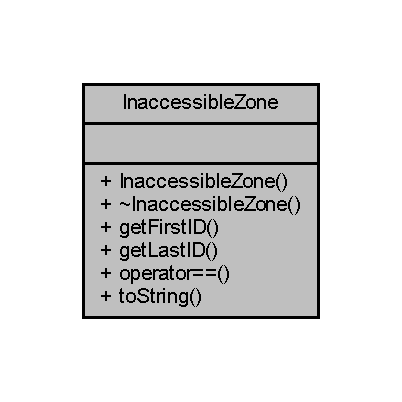
\includegraphics[width=193pt]{class_inaccessible_zone__coll__graph}
\end{center}
\end{figure}
\subsection*{Membros públicos}
\begin{DoxyCompactItemize}
\item 
\hypertarget{class_inaccessible_zone_ac571011fba0cd079537990d67e5199fa}{}{\bfseries Inaccessible\+Zone} (int node1, int node2)\label{class_inaccessible_zone_ac571011fba0cd079537990d67e5199fa}

\item 
\hypertarget{class_inaccessible_zone_a409eaa2fbfb3f84317a89c81e07dbafe}{}int {\bfseries get\+First\+I\+D} () const \label{class_inaccessible_zone_a409eaa2fbfb3f84317a89c81e07dbafe}

\item 
\hypertarget{class_inaccessible_zone_ad797feb433c52fc0922ce166d4a6df1e}{}int {\bfseries get\+Last\+I\+D} () const \label{class_inaccessible_zone_ad797feb433c52fc0922ce166d4a6df1e}

\item 
\hypertarget{class_inaccessible_zone_a02480a51fb032c5fee74fab422fe5166}{}bool {\bfseries operator==} (const \hyperlink{class_inaccessible_zone}{Inaccessible\+Zone} \&rv)\label{class_inaccessible_zone_a02480a51fb032c5fee74fab422fe5166}

\item 
\hypertarget{class_inaccessible_zone_a1f6e8009d1892572c7072e4fb8bb1d31}{}string {\bfseries to\+String} () const \label{class_inaccessible_zone_a1f6e8009d1892572c7072e4fb8bb1d31}

\end{DoxyCompactItemize}


A documentação para esta classe foi gerada a partir dos seguintes ficheiros\+:\begin{DoxyCompactItemize}
\item 
C\+:/\+Users/josea/\+Documents/\+Git\+Hub/\+C\+A\+L-\/\+Proj/\+Easy\+Pilot/src/Utilities.\+h\item 
C\+:/\+Users/josea/\+Documents/\+Git\+Hub/\+C\+A\+L-\/\+Proj/\+Easy\+Pilot/src/Utilities.\+cpp\end{DoxyCompactItemize}

\hypertarget{classstd_1_1_invalid_input}{}\section{Referência à classe std\+:\+:Invalid\+Input}
\label{classstd_1_1_invalid_input}\index{std\+::\+Invalid\+Input@{std\+::\+Invalid\+Input}}


{\ttfamily \#include $<$Menu\+Manager.\+h$>$}



Diagrama de colaboração para std\+:\+:Invalid\+Input\+:
\nopagebreak
\begin{figure}[H]
\begin{center}
\leavevmode
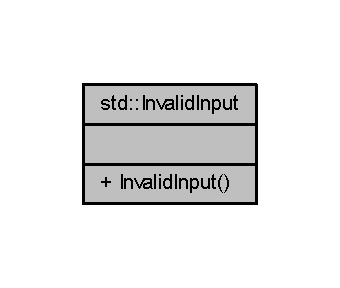
\includegraphics[width=163pt]{classstd_1_1_invalid_input__coll__graph}
\end{center}
\end{figure}
\subsection*{Membros públicos}
\begin{DoxyCompactItemize}
\item 
\hyperlink{classstd_1_1_invalid_input_ad85ad7bbb3d6bbcaa3d8071f69cdcbd1}{Invalid\+Input} ()
\end{DoxyCompactItemize}


\subsection{Documentação dos Construtores \& Destrutor}
\hypertarget{classstd_1_1_invalid_input_ad85ad7bbb3d6bbcaa3d8071f69cdcbd1}{}\index{std\+::\+Invalid\+Input@{std\+::\+Invalid\+Input}!Invalid\+Input@{Invalid\+Input}}
\index{Invalid\+Input@{Invalid\+Input}!std\+::\+Invalid\+Input@{std\+::\+Invalid\+Input}}
\subsubsection[{Invalid\+Input()}]{\setlength{\rightskip}{0pt plus 5cm}std\+::\+Invalid\+Input\+::\+Invalid\+Input (
\begin{DoxyParamCaption}
{}
\end{DoxyParamCaption}
)\hspace{0.3cm}{\ttfamily [inline]}}\label{classstd_1_1_invalid_input_ad85ad7bbb3d6bbcaa3d8071f69cdcbd1}


A documentação para esta classe foi gerada a partir do seguinte ficheiro\+:\begin{DoxyCompactItemize}
\item 
C\+:/\+Users/josea/\+Documents/\+Git\+Hub/\+C\+A\+L-\/\+Easy\+Pilot/\+Easy\+Pilot/src/\hyperlink{_menu_manager_8h}{Menu\+Manager.\+h}\end{DoxyCompactItemize}

\hypertarget{struct_limit_coords}{}\section{Referência à estrutura Limit\+Coords}
\label{struct_limit_coords}\index{Limit\+Coords@{Limit\+Coords}}


{\ttfamily \#include $<$Easy\+Pilot.\+h$>$}



Diagrama de colaboração para Limit\+Coords\+:
\nopagebreak
\begin{figure}[H]
\begin{center}
\leavevmode
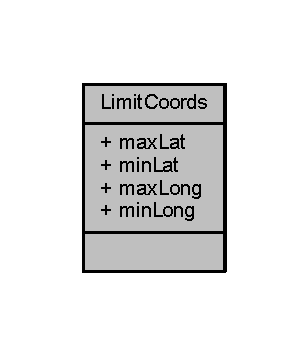
\includegraphics[width=148pt]{struct_limit_coords__coll__graph}
\end{center}
\end{figure}
\subsection*{Atributos Públicos}
\begin{DoxyCompactItemize}
\item 
\hypertarget{struct_limit_coords_a9a0fcf9e011923cb568a1c584a51f654}{}double {\bfseries max\+Lat}\label{struct_limit_coords_a9a0fcf9e011923cb568a1c584a51f654}

\item 
\hypertarget{struct_limit_coords_a1a647ec24500cd353ef30d0de159f0be}{}double {\bfseries min\+Lat}\label{struct_limit_coords_a1a647ec24500cd353ef30d0de159f0be}

\item 
\hypertarget{struct_limit_coords_aeaddaee7845266a6f234ffd50f748ae4}{}double {\bfseries max\+Long}\label{struct_limit_coords_aeaddaee7845266a6f234ffd50f748ae4}

\item 
\hypertarget{struct_limit_coords_a3ef4041cf2ffec8011de8ff137180895}{}double {\bfseries min\+Long}\label{struct_limit_coords_a3ef4041cf2ffec8011de8ff137180895}

\end{DoxyCompactItemize}


\subsection{Descrição detalhada}
\hyperlink{struct_limit_coords}{Limit\+Coords} will store the highest and lowest longitude and latitude of the nodes 

A documentação para esta estrutura foi gerada a partir do seguinte ficheiro\+:\begin{DoxyCompactItemize}
\item 
C\+:/\+Users/josea/\+Documents/\+Git\+Hub/\+C\+A\+L-\/\+Proj/\+Easy\+Pilot/src/Easy\+Pilot.\+h\end{DoxyCompactItemize}

\hypertarget{class_link}{}\section{Referência à classe Link}
\label{class_link}\index{Link@{Link}}


{\ttfamily \#include $<$Utilities.\+h$>$}



Diagrama de colaboração para Link\+:
\nopagebreak
\begin{figure}[H]
\begin{center}
\leavevmode
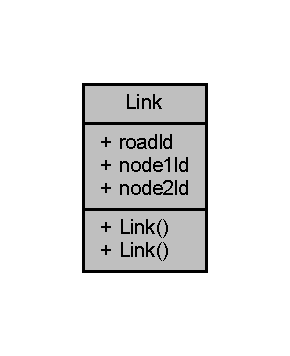
\includegraphics[width=139pt]{class_link__coll__graph}
\end{center}
\end{figure}
\subsection*{Membros públicos}
\begin{DoxyCompactItemize}
\item 
\hyperlink{class_link_a1918a8473cee40bbed17b8e926cb85d9}{Link} ()
\item 
\hyperlink{class_link_adb501ce3d816ea3a7dd603aa97c8bce6}{Link} (unsigned r, unsigned n1, unsigned n2)
\end{DoxyCompactItemize}
\subsection*{Atributos Públicos}
\begin{DoxyCompactItemize}
\item 
unsigned \hyperlink{class_link_a933579cb192194d9158937143e8ab970}{road\+Id}
\item 
unsigned \hyperlink{class_link_ac2104772717d9ece063ebd9bac18f4e0}{node1\+Id}
\item 
unsigned \hyperlink{class_link_a7d3bd226ba9935e42424a296cad221ba}{node2\+Id}
\end{DoxyCompactItemize}


\subsection{Documentação dos Construtores \& Destrutor}
\hypertarget{class_link_a1918a8473cee40bbed17b8e926cb85d9}{}\index{Link@{Link}!Link@{Link}}
\index{Link@{Link}!Link@{Link}}
\subsubsection[{Link()}]{\setlength{\rightskip}{0pt plus 5cm}Link\+::\+Link (
\begin{DoxyParamCaption}
{}
\end{DoxyParamCaption}
)\hspace{0.3cm}{\ttfamily [inline]}}\label{class_link_a1918a8473cee40bbed17b8e926cb85d9}
\hypertarget{class_link_adb501ce3d816ea3a7dd603aa97c8bce6}{}\index{Link@{Link}!Link@{Link}}
\index{Link@{Link}!Link@{Link}}
\subsubsection[{Link(unsigned r, unsigned n1, unsigned n2)}]{\setlength{\rightskip}{0pt plus 5cm}Link\+::\+Link (
\begin{DoxyParamCaption}
\item[{unsigned}]{r, }
\item[{unsigned}]{n1, }
\item[{unsigned}]{n2}
\end{DoxyParamCaption}
)\hspace{0.3cm}{\ttfamily [inline]}}\label{class_link_adb501ce3d816ea3a7dd603aa97c8bce6}


\subsection{Documentação dos dados membro}
\hypertarget{class_link_ac2104772717d9ece063ebd9bac18f4e0}{}\index{Link@{Link}!node1\+Id@{node1\+Id}}
\index{node1\+Id@{node1\+Id}!Link@{Link}}
\subsubsection[{node1\+Id}]{\setlength{\rightskip}{0pt plus 5cm}unsigned Link\+::node1\+Id}\label{class_link_ac2104772717d9ece063ebd9bac18f4e0}
\hypertarget{class_link_a7d3bd226ba9935e42424a296cad221ba}{}\index{Link@{Link}!node2\+Id@{node2\+Id}}
\index{node2\+Id@{node2\+Id}!Link@{Link}}
\subsubsection[{node2\+Id}]{\setlength{\rightskip}{0pt plus 5cm}unsigned Link\+::node2\+Id}\label{class_link_a7d3bd226ba9935e42424a296cad221ba}
\hypertarget{class_link_a933579cb192194d9158937143e8ab970}{}\index{Link@{Link}!road\+Id@{road\+Id}}
\index{road\+Id@{road\+Id}!Link@{Link}}
\subsubsection[{road\+Id}]{\setlength{\rightskip}{0pt plus 5cm}unsigned Link\+::road\+Id}\label{class_link_a933579cb192194d9158937143e8ab970}


A documentação para esta classe foi gerada a partir do seguinte ficheiro\+:\begin{DoxyCompactItemize}
\item 
C\+:/\+Users/josea/\+Documents/\+Git\+Hub/\+C\+A\+L-\/\+Easy\+Pilot/\+Easy\+Pilot/src/\hyperlink{_utilities_8h}{Utilities.\+h}\end{DoxyCompactItemize}

\hypertarget{classstd_1_1_menu_manager}{}\section{Referência à classe std\+:\+:Menu\+Manager}
\label{classstd_1_1_menu_manager}\index{std\+::\+Menu\+Manager@{std\+::\+Menu\+Manager}}


{\ttfamily \#include $<$Menu\+Manager.\+h$>$}



Diagrama de colaboração para std\+:\+:Menu\+Manager\+:
\nopagebreak
\begin{figure}[H]
\begin{center}
\leavevmode
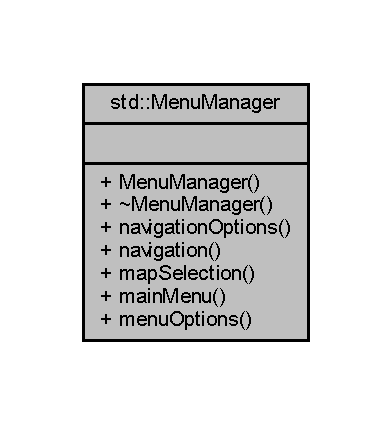
\includegraphics[width=238pt]{classstd_1_1_menu_manager__coll__graph}
\end{center}
\end{figure}
\subsection*{Membros públicos}
\begin{DoxyCompactItemize}
\item 
\hyperlink{classstd_1_1_menu_manager_a0e57899dfa981f18aa39890638a0d131}{Menu\+Manager} ()
\item 
virtual \hyperlink{classstd_1_1_menu_manager_a2e39acf092dd4a46e904ca141088bcd1}{$\sim$\+Menu\+Manager} ()
\item 
void \hyperlink{classstd_1_1_menu_manager_a6b49d6cd4fe3260d9642dbb20381f43c}{navigation\+Options} (\hyperlink{class_easy_pilot}{Easy\+Pilot} $\ast$gps)
\item 
void \hyperlink{classstd_1_1_menu_manager_a07bff9624aa3fc9104ec98c79b8c37a1}{navigation} (\hyperlink{class_easy_pilot}{Easy\+Pilot} $\ast$gps)
\item 
void \hyperlink{classstd_1_1_menu_manager_a77cd2018d2592e12d39dd07eb6f21022}{map\+Selection} (\hyperlink{class_easy_pilot}{Easy\+Pilot} $\ast$gps)
\item 
void \hyperlink{classstd_1_1_menu_manager_a638c286f464bf2d495aa2b4fb213302e}{main\+Menu} (\hyperlink{class_easy_pilot}{Easy\+Pilot} $\ast$gps)
\item 
void \hyperlink{classstd_1_1_menu_manager_abed94057ed99af5fc35be97742359585}{Approximate\+District\+Selection} (\hyperlink{class_easy_pilot}{Easy\+Pilot} $\ast$gps)
\item 
void \hyperlink{classstd_1_1_menu_manager_a9d27786670fa4ccfec164863eec87b4a}{Exact\+District\+Selection} (\hyperlink{class_easy_pilot}{Easy\+Pilot} $\ast$gps)
\item 
void \hyperlink{classstd_1_1_menu_manager_aa15f39e5d4c32479e5487be2e1b38d67}{Approximate\+Dest\+Selection} (\hyperlink{class_easy_pilot}{Easy\+Pilot} $\ast$gps)
\item 
void \hyperlink{classstd_1_1_menu_manager_a2ffb71762aba39d2d9e0233e7bc88f92}{Exact\+Dest\+Selection} (\hyperlink{class_easy_pilot}{Easy\+Pilot} $\ast$gps)
\item 
void \hyperlink{classstd_1_1_menu_manager_a430a4b321213835da37750a9bd565865}{input\+Options} (\hyperlink{class_easy_pilot}{Easy\+Pilot} $\ast$gps)
\item 
int \hyperlink{classstd_1_1_menu_manager_a1235a2b53d90aeb5f60c043be9caf62b}{menu\+Options} (vector$<$ string $>$ options)
\end{DoxyCompactItemize}


\subsection{Documentação dos Construtores \& Destrutor}
\hypertarget{classstd_1_1_menu_manager_a0e57899dfa981f18aa39890638a0d131}{}\index{std\+::\+Menu\+Manager@{std\+::\+Menu\+Manager}!Menu\+Manager@{Menu\+Manager}}
\index{Menu\+Manager@{Menu\+Manager}!std\+::\+Menu\+Manager@{std\+::\+Menu\+Manager}}
\subsubsection[{Menu\+Manager()}]{\setlength{\rightskip}{0pt plus 5cm}std\+::\+Menu\+Manager\+::\+Menu\+Manager (
\begin{DoxyParamCaption}
{}
\end{DoxyParamCaption}
)}\label{classstd_1_1_menu_manager_a0e57899dfa981f18aa39890638a0d131}
\hypertarget{classstd_1_1_menu_manager_a2e39acf092dd4a46e904ca141088bcd1}{}\index{std\+::\+Menu\+Manager@{std\+::\+Menu\+Manager}!````~Menu\+Manager@{$\sim$\+Menu\+Manager}}
\index{````~Menu\+Manager@{$\sim$\+Menu\+Manager}!std\+::\+Menu\+Manager@{std\+::\+Menu\+Manager}}
\subsubsection[{$\sim$\+Menu\+Manager()}]{\setlength{\rightskip}{0pt plus 5cm}std\+::\+Menu\+Manager\+::$\sim$\+Menu\+Manager (
\begin{DoxyParamCaption}
{}
\end{DoxyParamCaption}
)\hspace{0.3cm}{\ttfamily [virtual]}}\label{classstd_1_1_menu_manager_a2e39acf092dd4a46e904ca141088bcd1}


\subsection{Documentação dos métodos}
\hypertarget{classstd_1_1_menu_manager_aa15f39e5d4c32479e5487be2e1b38d67}{}\index{std\+::\+Menu\+Manager@{std\+::\+Menu\+Manager}!Approximate\+Dest\+Selection@{Approximate\+Dest\+Selection}}
\index{Approximate\+Dest\+Selection@{Approximate\+Dest\+Selection}!std\+::\+Menu\+Manager@{std\+::\+Menu\+Manager}}
\subsubsection[{Approximate\+Dest\+Selection(\+Easy\+Pilot $\ast$gps)}]{\setlength{\rightskip}{0pt plus 5cm}void Menu\+Manager\+::\+Approximate\+Dest\+Selection (
\begin{DoxyParamCaption}
\item[{{\bf Easy\+Pilot} $\ast$}]{gps}
\end{DoxyParamCaption}
)}\label{classstd_1_1_menu_manager_aa15f39e5d4c32479e5487be2e1b38d67}
\hypertarget{classstd_1_1_menu_manager_abed94057ed99af5fc35be97742359585}{}\index{std\+::\+Menu\+Manager@{std\+::\+Menu\+Manager}!Approximate\+District\+Selection@{Approximate\+District\+Selection}}
\index{Approximate\+District\+Selection@{Approximate\+District\+Selection}!std\+::\+Menu\+Manager@{std\+::\+Menu\+Manager}}
\subsubsection[{Approximate\+District\+Selection(\+Easy\+Pilot $\ast$gps)}]{\setlength{\rightskip}{0pt plus 5cm}void Menu\+Manager\+::\+Approximate\+District\+Selection (
\begin{DoxyParamCaption}
\item[{{\bf Easy\+Pilot} $\ast$}]{gps}
\end{DoxyParamCaption}
)}\label{classstd_1_1_menu_manager_abed94057ed99af5fc35be97742359585}
\hypertarget{classstd_1_1_menu_manager_a2ffb71762aba39d2d9e0233e7bc88f92}{}\index{std\+::\+Menu\+Manager@{std\+::\+Menu\+Manager}!Exact\+Dest\+Selection@{Exact\+Dest\+Selection}}
\index{Exact\+Dest\+Selection@{Exact\+Dest\+Selection}!std\+::\+Menu\+Manager@{std\+::\+Menu\+Manager}}
\subsubsection[{Exact\+Dest\+Selection(\+Easy\+Pilot $\ast$gps)}]{\setlength{\rightskip}{0pt plus 5cm}void Menu\+Manager\+::\+Exact\+Dest\+Selection (
\begin{DoxyParamCaption}
\item[{{\bf Easy\+Pilot} $\ast$}]{gps}
\end{DoxyParamCaption}
)}\label{classstd_1_1_menu_manager_a2ffb71762aba39d2d9e0233e7bc88f92}
\hypertarget{classstd_1_1_menu_manager_a9d27786670fa4ccfec164863eec87b4a}{}\index{std\+::\+Menu\+Manager@{std\+::\+Menu\+Manager}!Exact\+District\+Selection@{Exact\+District\+Selection}}
\index{Exact\+District\+Selection@{Exact\+District\+Selection}!std\+::\+Menu\+Manager@{std\+::\+Menu\+Manager}}
\subsubsection[{Exact\+District\+Selection(\+Easy\+Pilot $\ast$gps)}]{\setlength{\rightskip}{0pt plus 5cm}void Menu\+Manager\+::\+Exact\+District\+Selection (
\begin{DoxyParamCaption}
\item[{{\bf Easy\+Pilot} $\ast$}]{gps}
\end{DoxyParamCaption}
)}\label{classstd_1_1_menu_manager_a9d27786670fa4ccfec164863eec87b4a}
\hypertarget{classstd_1_1_menu_manager_a430a4b321213835da37750a9bd565865}{}\index{std\+::\+Menu\+Manager@{std\+::\+Menu\+Manager}!input\+Options@{input\+Options}}
\index{input\+Options@{input\+Options}!std\+::\+Menu\+Manager@{std\+::\+Menu\+Manager}}
\subsubsection[{input\+Options(\+Easy\+Pilot $\ast$gps)}]{\setlength{\rightskip}{0pt plus 5cm}void Menu\+Manager\+::input\+Options (
\begin{DoxyParamCaption}
\item[{{\bf Easy\+Pilot} $\ast$}]{gps}
\end{DoxyParamCaption}
)}\label{classstd_1_1_menu_manager_a430a4b321213835da37750a9bd565865}
\hypertarget{classstd_1_1_menu_manager_a638c286f464bf2d495aa2b4fb213302e}{}\index{std\+::\+Menu\+Manager@{std\+::\+Menu\+Manager}!main\+Menu@{main\+Menu}}
\index{main\+Menu@{main\+Menu}!std\+::\+Menu\+Manager@{std\+::\+Menu\+Manager}}
\subsubsection[{main\+Menu(\+Easy\+Pilot $\ast$gps)}]{\setlength{\rightskip}{0pt plus 5cm}void Menu\+Manager\+::main\+Menu (
\begin{DoxyParamCaption}
\item[{{\bf Easy\+Pilot} $\ast$}]{gps}
\end{DoxyParamCaption}
)}\label{classstd_1_1_menu_manager_a638c286f464bf2d495aa2b4fb213302e}
\hypertarget{classstd_1_1_menu_manager_a77cd2018d2592e12d39dd07eb6f21022}{}\index{std\+::\+Menu\+Manager@{std\+::\+Menu\+Manager}!map\+Selection@{map\+Selection}}
\index{map\+Selection@{map\+Selection}!std\+::\+Menu\+Manager@{std\+::\+Menu\+Manager}}
\subsubsection[{map\+Selection(\+Easy\+Pilot $\ast$gps)}]{\setlength{\rightskip}{0pt plus 5cm}void Menu\+Manager\+::map\+Selection (
\begin{DoxyParamCaption}
\item[{{\bf Easy\+Pilot} $\ast$}]{gps}
\end{DoxyParamCaption}
)}\label{classstd_1_1_menu_manager_a77cd2018d2592e12d39dd07eb6f21022}
\hypertarget{classstd_1_1_menu_manager_a1235a2b53d90aeb5f60c043be9caf62b}{}\index{std\+::\+Menu\+Manager@{std\+::\+Menu\+Manager}!menu\+Options@{menu\+Options}}
\index{menu\+Options@{menu\+Options}!std\+::\+Menu\+Manager@{std\+::\+Menu\+Manager}}
\subsubsection[{menu\+Options(vector$<$ string $>$ options)}]{\setlength{\rightskip}{0pt plus 5cm}int Menu\+Manager\+::menu\+Options (
\begin{DoxyParamCaption}
\item[{vector$<$ string $>$}]{options}
\end{DoxyParamCaption}
)}\label{classstd_1_1_menu_manager_a1235a2b53d90aeb5f60c043be9caf62b}
\hypertarget{classstd_1_1_menu_manager_a07bff9624aa3fc9104ec98c79b8c37a1}{}\index{std\+::\+Menu\+Manager@{std\+::\+Menu\+Manager}!navigation@{navigation}}
\index{navigation@{navigation}!std\+::\+Menu\+Manager@{std\+::\+Menu\+Manager}}
\subsubsection[{navigation(\+Easy\+Pilot $\ast$gps)}]{\setlength{\rightskip}{0pt plus 5cm}void Menu\+Manager\+::navigation (
\begin{DoxyParamCaption}
\item[{{\bf Easy\+Pilot} $\ast$}]{gps}
\end{DoxyParamCaption}
)}\label{classstd_1_1_menu_manager_a07bff9624aa3fc9104ec98c79b8c37a1}
\hypertarget{classstd_1_1_menu_manager_a6b49d6cd4fe3260d9642dbb20381f43c}{}\index{std\+::\+Menu\+Manager@{std\+::\+Menu\+Manager}!navigation\+Options@{navigation\+Options}}
\index{navigation\+Options@{navigation\+Options}!std\+::\+Menu\+Manager@{std\+::\+Menu\+Manager}}
\subsubsection[{navigation\+Options(\+Easy\+Pilot $\ast$gps)}]{\setlength{\rightskip}{0pt plus 5cm}void Menu\+Manager\+::navigation\+Options (
\begin{DoxyParamCaption}
\item[{{\bf Easy\+Pilot} $\ast$}]{gps}
\end{DoxyParamCaption}
)}\label{classstd_1_1_menu_manager_a6b49d6cd4fe3260d9642dbb20381f43c}


A documentação para esta classe foi gerada a partir dos seguintes ficheiros\+:\begin{DoxyCompactItemize}
\item 
C\+:/\+Users/josea/\+Documents/\+Git\+Hub/\+C\+A\+L-\/\+Easy\+Pilot/\+Easy\+Pilot/src/\hyperlink{_menu_manager_8h}{Menu\+Manager.\+h}\item 
C\+:/\+Users/josea/\+Documents/\+Git\+Hub/\+C\+A\+L-\/\+Easy\+Pilot/\+Easy\+Pilot/src/\hyperlink{_menu_manager_8cpp}{Menu\+Manager.\+cpp}\end{DoxyCompactItemize}

\hypertarget{class_toll}{}\section{Referência à classe Toll}
\label{class_toll}\index{Toll@{Toll}}


Diagrama de colaboração para Toll\+:
\nopagebreak
\begin{figure}[H]
\begin{center}
\leavevmode
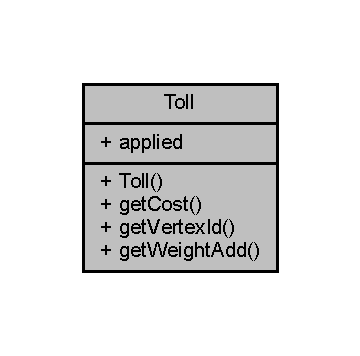
\includegraphics[width=173pt]{class_toll__coll__graph}
\end{center}
\end{figure}
\subsection*{Membros públicos}
\begin{DoxyCompactItemize}
\item 
\hypertarget{class_toll_ae7ee55783fc26b0f68a91586e7238a2c}{}{\bfseries Toll} (int vertex\+I\+D, float cost)\label{class_toll_ae7ee55783fc26b0f68a91586e7238a2c}

\item 
\hypertarget{class_toll_a09a987b280dada924f83ca07669f3a9b}{}float {\bfseries get\+Cost} () const \label{class_toll_a09a987b280dada924f83ca07669f3a9b}

\item 
\hypertarget{class_toll_a9b206f487334ea8930a9be1b06e14ca4}{}int {\bfseries get\+Vertex\+Id} () const \label{class_toll_a9b206f487334ea8930a9be1b06e14ca4}

\item 
\hypertarget{class_toll_a5cd8903fb8bfdd46b726291e3409e915}{}int {\bfseries get\+Weight\+Add} () const \label{class_toll_a5cd8903fb8bfdd46b726291e3409e915}

\end{DoxyCompactItemize}
\subsection*{Atributos Públicos}
\begin{DoxyCompactItemize}
\item 
\hypertarget{class_toll_a2744c563ee9430acf43cb8ed92cf44d9}{}bool {\bfseries applied}\label{class_toll_a2744c563ee9430acf43cb8ed92cf44d9}

\end{DoxyCompactItemize}


A documentação para esta classe foi gerada a partir dos seguintes ficheiros\+:\begin{DoxyCompactItemize}
\item 
C\+:/\+Users/josea/\+Documents/\+Git\+Hub/\+C\+A\+L-\/\+Proj/\+Easy\+Pilot/src/Utilities.\+h\item 
C\+:/\+Users/josea/\+Documents/\+Git\+Hub/\+C\+A\+L-\/\+Proj/\+Easy\+Pilot/src/Utilities.\+cpp\end{DoxyCompactItemize}

\hypertarget{class_vertex}{}\section{Referência à classe Template Vertex$<$ T $>$}
\label{class_vertex}\index{Vertex$<$ T $>$@{Vertex$<$ T $>$}}


{\ttfamily \#include $<$Graph.\+h$>$}



Diagrama de colaboração para Vertex$<$ T $>$\+:
\nopagebreak
\begin{figure}[H]
\begin{center}
\leavevmode
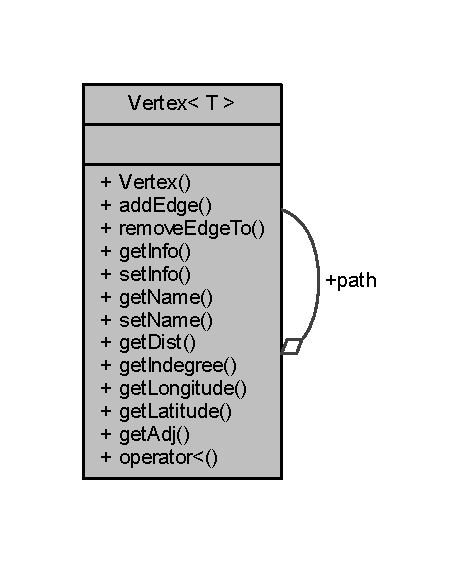
\includegraphics[width=221pt]{class_vertex__coll__graph}
\end{center}
\end{figure}
\subsection*{Membros públicos}
\begin{DoxyCompactItemize}
\item 
\hyperlink{class_vertex_a32481367e36d2162714bc411f31b5f8f}{Vertex} (T in, double longitude, double latitude)
\item 
void \hyperlink{class_vertex_a40b147df89a89885a06fd9c3912c6dd5}{add\+Edge} (\hyperlink{class_vertex}{Vertex}$<$ T $>$ $\ast$dest, double w, bool tw, bool blocked, T id, string name)
\item 
bool \hyperlink{class_vertex_ab2b5b43fb1709a901b78718436763a84}{remove\+Edge\+To} (\hyperlink{class_vertex}{Vertex}$<$ T $>$ $\ast$d)
\item 
T \hyperlink{class_vertex_a5880b4b252ae6818819c2f9645784b59}{get\+Info} () const 
\item 
void \hyperlink{class_vertex_a31cd60c26640f8072a928ba70eb2f95e}{set\+Info} (T info)
\item 
string \hyperlink{class_vertex_a878c08e3eca2b53b173fa8c1fa77227d}{get\+Name} () const 
\item 
void \hyperlink{class_vertex_aee1d15f2efc9c7baecff72265beb1acf}{set\+Name} (string name)
\item 
int \hyperlink{class_vertex_a3379c6cbcf1eaacc098381e3557a0b52}{get\+Dist} () const 
\item 
int \hyperlink{class_vertex_a305ef01582f945f22134abb9294fe1f3}{get\+Indegree} () const 
\item 
double \hyperlink{class_vertex_aa88dbd3c9af86b1fd567a43c0da69017}{get\+Longitude} () const 
\item 
double \hyperlink{class_vertex_afbf6474fe17f4fd509bda1026fd81385}{get\+Latitude} () const 
\item 
vector$<$ \hyperlink{class_edge}{Edge}$<$ T $>$ $>$ \hyperlink{class_vertex_a4d8021f4861cc4195af3ecf042a015cc}{get\+Adj} () const 
\item 
bool \hyperlink{class_vertex_a7091b26f281a5041b1775a3d3f9cb7a6}{operator$<$} (const \hyperlink{class_vertex}{Vertex}$<$ T $>$ vertex)
\end{DoxyCompactItemize}
\subsection*{Atributos Públicos}
\begin{DoxyCompactItemize}
\item 
\hyperlink{class_vertex}{Vertex} $\ast$ \hyperlink{class_vertex_abd40febd917aa25add6bd42237c8463a}{path}
\end{DoxyCompactItemize}
\subsection*{Amigos}
\begin{DoxyCompactItemize}
\item 
class \hyperlink{class_vertex_aefa9b76cd57411c5354e5620dc2d84dd}{Graph$<$ T $>$}
\end{DoxyCompactItemize}


\subsection{Documentação dos Construtores \& Destrutor}
\hypertarget{class_vertex_a32481367e36d2162714bc411f31b5f8f}{}\index{Vertex@{Vertex}!Vertex@{Vertex}}
\index{Vertex@{Vertex}!Vertex@{Vertex}}
\subsubsection[{Vertex(\+T in, double longitude, double latitude)}]{\setlength{\rightskip}{0pt plus 5cm}template$<$class T $>$ {\bf Vertex}$<$ T $>$\+::{\bf Vertex} (
\begin{DoxyParamCaption}
\item[{T}]{in, }
\item[{double}]{longitude, }
\item[{double}]{latitude}
\end{DoxyParamCaption}
)}\label{class_vertex_a32481367e36d2162714bc411f31b5f8f}


\subsection{Documentação dos métodos}
\hypertarget{class_vertex_a40b147df89a89885a06fd9c3912c6dd5}{}\index{Vertex@{Vertex}!add\+Edge@{add\+Edge}}
\index{add\+Edge@{add\+Edge}!Vertex@{Vertex}}
\subsubsection[{add\+Edge(\+Vertex$<$ T $>$ $\ast$dest, double w, bool tw, bool blocked, T id, string name)}]{\setlength{\rightskip}{0pt plus 5cm}template$<$class T $>$ void {\bf Vertex}$<$ T $>$\+::add\+Edge (
\begin{DoxyParamCaption}
\item[{{\bf Vertex}$<$ T $>$ $\ast$}]{dest, }
\item[{double}]{w, }
\item[{bool}]{tw, }
\item[{bool}]{blocked, }
\item[{T}]{id, }
\item[{string}]{name}
\end{DoxyParamCaption}
)}\label{class_vertex_a40b147df89a89885a06fd9c3912c6dd5}
\hypertarget{class_vertex_a4d8021f4861cc4195af3ecf042a015cc}{}\index{Vertex@{Vertex}!get\+Adj@{get\+Adj}}
\index{get\+Adj@{get\+Adj}!Vertex@{Vertex}}
\subsubsection[{get\+Adj() const }]{\setlength{\rightskip}{0pt plus 5cm}template$<$class T $>$ vector$<$ {\bf Edge}$<$ T $>$ $>$ {\bf Vertex}$<$ T $>$\+::get\+Adj (
\begin{DoxyParamCaption}
{}
\end{DoxyParamCaption}
) const}\label{class_vertex_a4d8021f4861cc4195af3ecf042a015cc}
\hypertarget{class_vertex_a3379c6cbcf1eaacc098381e3557a0b52}{}\index{Vertex@{Vertex}!get\+Dist@{get\+Dist}}
\index{get\+Dist@{get\+Dist}!Vertex@{Vertex}}
\subsubsection[{get\+Dist() const }]{\setlength{\rightskip}{0pt plus 5cm}template$<$class T $>$ int {\bf Vertex}$<$ T $>$\+::get\+Dist (
\begin{DoxyParamCaption}
{}
\end{DoxyParamCaption}
) const}\label{class_vertex_a3379c6cbcf1eaacc098381e3557a0b52}
\hypertarget{class_vertex_a305ef01582f945f22134abb9294fe1f3}{}\index{Vertex@{Vertex}!get\+Indegree@{get\+Indegree}}
\index{get\+Indegree@{get\+Indegree}!Vertex@{Vertex}}
\subsubsection[{get\+Indegree() const }]{\setlength{\rightskip}{0pt plus 5cm}template$<$class T $>$ int {\bf Vertex}$<$ T $>$\+::get\+Indegree (
\begin{DoxyParamCaption}
{}
\end{DoxyParamCaption}
) const}\label{class_vertex_a305ef01582f945f22134abb9294fe1f3}
\hypertarget{class_vertex_a5880b4b252ae6818819c2f9645784b59}{}\index{Vertex@{Vertex}!get\+Info@{get\+Info}}
\index{get\+Info@{get\+Info}!Vertex@{Vertex}}
\subsubsection[{get\+Info() const }]{\setlength{\rightskip}{0pt plus 5cm}template$<$class T $>$ T {\bf Vertex}$<$ T $>$\+::get\+Info (
\begin{DoxyParamCaption}
{}
\end{DoxyParamCaption}
) const}\label{class_vertex_a5880b4b252ae6818819c2f9645784b59}
\hypertarget{class_vertex_afbf6474fe17f4fd509bda1026fd81385}{}\index{Vertex@{Vertex}!get\+Latitude@{get\+Latitude}}
\index{get\+Latitude@{get\+Latitude}!Vertex@{Vertex}}
\subsubsection[{get\+Latitude() const }]{\setlength{\rightskip}{0pt plus 5cm}template$<$class T $>$ double {\bf Vertex}$<$ T $>$\+::get\+Latitude (
\begin{DoxyParamCaption}
{}
\end{DoxyParamCaption}
) const}\label{class_vertex_afbf6474fe17f4fd509bda1026fd81385}
\hypertarget{class_vertex_aa88dbd3c9af86b1fd567a43c0da69017}{}\index{Vertex@{Vertex}!get\+Longitude@{get\+Longitude}}
\index{get\+Longitude@{get\+Longitude}!Vertex@{Vertex}}
\subsubsection[{get\+Longitude() const }]{\setlength{\rightskip}{0pt plus 5cm}template$<$class T $>$ double {\bf Vertex}$<$ T $>$\+::get\+Longitude (
\begin{DoxyParamCaption}
{}
\end{DoxyParamCaption}
) const}\label{class_vertex_aa88dbd3c9af86b1fd567a43c0da69017}
\hypertarget{class_vertex_a878c08e3eca2b53b173fa8c1fa77227d}{}\index{Vertex@{Vertex}!get\+Name@{get\+Name}}
\index{get\+Name@{get\+Name}!Vertex@{Vertex}}
\subsubsection[{get\+Name() const }]{\setlength{\rightskip}{0pt plus 5cm}template$<$class T $>$ string {\bf Vertex}$<$ T $>$\+::get\+Name (
\begin{DoxyParamCaption}
{}
\end{DoxyParamCaption}
) const}\label{class_vertex_a878c08e3eca2b53b173fa8c1fa77227d}
\hypertarget{class_vertex_a7091b26f281a5041b1775a3d3f9cb7a6}{}\index{Vertex@{Vertex}!operator$<$@{operator$<$}}
\index{operator$<$@{operator$<$}!Vertex@{Vertex}}
\subsubsection[{operator$<$(const Vertex$<$ T $>$ vertex)}]{\setlength{\rightskip}{0pt plus 5cm}template$<$class T$>$ bool {\bf Vertex}$<$ T $>$\+::operator$<$ (
\begin{DoxyParamCaption}
\item[{const {\bf Vertex}$<$ T $>$}]{vertex}
\end{DoxyParamCaption}
)}\label{class_vertex_a7091b26f281a5041b1775a3d3f9cb7a6}
\hypertarget{class_vertex_ab2b5b43fb1709a901b78718436763a84}{}\index{Vertex@{Vertex}!remove\+Edge\+To@{remove\+Edge\+To}}
\index{remove\+Edge\+To@{remove\+Edge\+To}!Vertex@{Vertex}}
\subsubsection[{remove\+Edge\+To(\+Vertex$<$ T $>$ $\ast$d)}]{\setlength{\rightskip}{0pt plus 5cm}template$<$class T $>$ bool {\bf Vertex}$<$ T $>$\+::remove\+Edge\+To (
\begin{DoxyParamCaption}
\item[{{\bf Vertex}$<$ T $>$ $\ast$}]{d}
\end{DoxyParamCaption}
)}\label{class_vertex_ab2b5b43fb1709a901b78718436763a84}
\hypertarget{class_vertex_a31cd60c26640f8072a928ba70eb2f95e}{}\index{Vertex@{Vertex}!set\+Info@{set\+Info}}
\index{set\+Info@{set\+Info}!Vertex@{Vertex}}
\subsubsection[{set\+Info(\+T info)}]{\setlength{\rightskip}{0pt plus 5cm}template$<$class T $>$ void {\bf Vertex}$<$ T $>$\+::set\+Info (
\begin{DoxyParamCaption}
\item[{T}]{info}
\end{DoxyParamCaption}
)}\label{class_vertex_a31cd60c26640f8072a928ba70eb2f95e}
\hypertarget{class_vertex_aee1d15f2efc9c7baecff72265beb1acf}{}\index{Vertex@{Vertex}!set\+Name@{set\+Name}}
\index{set\+Name@{set\+Name}!Vertex@{Vertex}}
\subsubsection[{set\+Name(string name)}]{\setlength{\rightskip}{0pt plus 5cm}template$<$class T $>$ void {\bf Vertex}$<$ T $>$\+::set\+Name (
\begin{DoxyParamCaption}
\item[{string}]{name}
\end{DoxyParamCaption}
)}\label{class_vertex_aee1d15f2efc9c7baecff72265beb1acf}


\subsection{Documentação das classes amigas e funções relacionadas}
\hypertarget{class_vertex_aefa9b76cd57411c5354e5620dc2d84dd}{}\index{Vertex@{Vertex}!Graph$<$ T $>$@{Graph$<$ T $>$}}
\index{Graph$<$ T $>$@{Graph$<$ T $>$}!Vertex@{Vertex}}
\subsubsection[{Graph$<$ T $>$}]{\setlength{\rightskip}{0pt plus 5cm}template$<$class T$>$ friend class {\bf Graph}$<$ T $>$\hspace{0.3cm}{\ttfamily [friend]}}\label{class_vertex_aefa9b76cd57411c5354e5620dc2d84dd}


\subsection{Documentação dos dados membro}
\hypertarget{class_vertex_abd40febd917aa25add6bd42237c8463a}{}\index{Vertex@{Vertex}!path@{path}}
\index{path@{path}!Vertex@{Vertex}}
\subsubsection[{path}]{\setlength{\rightskip}{0pt plus 5cm}template$<$class T$>$ {\bf Vertex}$\ast$ {\bf Vertex}$<$ T $>$\+::path}\label{class_vertex_abd40febd917aa25add6bd42237c8463a}


A documentação para esta classe foi gerada a partir do seguinte ficheiro\+:\begin{DoxyCompactItemize}
\item 
C\+:/\+Users/josea/\+Documents/\+Git\+Hub/\+C\+A\+L-\/\+Easy\+Pilot/\+Easy\+Pilot/src/\hyperlink{_graph_8h}{Graph.\+h}\end{DoxyCompactItemize}

\hypertarget{structvertex__greater__than}{}\section{Referência à estrutura Template vertex\+\_\+greater\+\_\+than$<$ T $>$}
\label{structvertex__greater__than}\index{vertex\+\_\+greater\+\_\+than$<$ T $>$@{vertex\+\_\+greater\+\_\+than$<$ T $>$}}


Diagrama de colaboração para vertex\+\_\+greater\+\_\+than$<$ T $>$\+:
\nopagebreak
\begin{figure}[H]
\begin{center}
\leavevmode
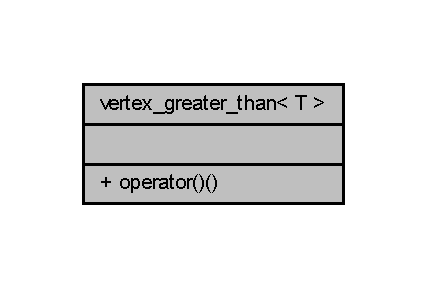
\includegraphics[width=205pt]{structvertex__greater__than__coll__graph}
\end{center}
\end{figure}
\subsection*{Membros públicos}
\begin{DoxyCompactItemize}
\item 
\hypertarget{structvertex__greater__than_af58940d572829488c2915ca53663631e}{}bool {\bfseries operator()} (\hyperlink{class_vertex}{Vertex}$<$ T $>$ $\ast$a, \hyperlink{class_vertex}{Vertex}$<$ T $>$ $\ast$b) const \label{structvertex__greater__than_af58940d572829488c2915ca53663631e}

\end{DoxyCompactItemize}


A documentação para esta estrutura foi gerada a partir do seguinte ficheiro\+:\begin{DoxyCompactItemize}
\item 
C\+:/\+Users/josea/\+Documents/\+Git\+Hub/\+C\+A\+L-\/\+Proj/\+Easy\+Pilot/src/Graph.\+h\end{DoxyCompactItemize}

%--- End generated contents ---

% Index
\backmatter
\newpage
\phantomsection
\clearemptydoublepage
\addcontentsline{toc}{chapter}{Índice}
\printindex

\end{document}
